%% ----------------------------------------------------------------
%% Thesis.tex -- MAIN FILE (the one that you compile with LaTeX)
%% ---------------------------------------------------------------- 

% Set up the document
\documentclass[a4paper, 12pt, oneside]{Thesis}  % Use the "Thesis" style, based on the ECS Thesis style by Steve Gunn
\graphicspath{Figures/}  % Location of the graphics files (set up for graphics to be in PDF format)

% Include any extra LaTeX packages required
\usepackage[square, numbers, comma, sort&compress]{natbib}  % Use the "Natbib" style for the references in the Bibliography
%\usepackage{biblatex}
\usepackage{verbatim}  % Needed for the "comment" environment to make LaTeX comments
\usepackage{vector}  % Allows "\bvec{}" and "\buvec{}" for "blackboard" style bold vectors in maths
\usepackage{graphics}
\usepackage{multirow}
\usepackage{epsfig}
\usepackage{float}
\usepackage{amsmath}
\usepackage{slashbox}
\usepackage{textcomp}
\usepackage[subfigure]{tocloft}
\usepackage{listings}
\usepackage[usenames,dvipsnames]{color} 		% Custom colors
\usepackage{notoccite}
\hypersetup{urlcolor=blue, colorlinks=true}  % Colours hyperlinks in blue, but this can be distracting if there are many links.

\renewcommand{\cftchapfont}{\bfseries}
\renewcommand{\cftchappagefont}{\bfseries}
\renewcommand{\cftchappresnum}{Chapter }
\renewcommand{\cftchapaftersnum}{:}
\renewcommand{\cftchapnumwidth}{6em}
\newcommand{\sub}[1]{\raisebox{-.4ex}{\scriptsize #1}}

\DeclareFontFamily{U}{euc}{}% I chose euc because the chart is called Euler cursive
\DeclareFontShape{U}{euc}{m}{n}{<-6>eurm5<6-8>eurm7<8->eurm10}{}%
\DeclareSymbolFont{AMSc}{U}{euc}{m}{n} % I chose AMSc because AMSa and AMSb are defined in the amsfonts-package
\DeclareMathSymbol{\umu}{\mathord}{AMSc}{"16} 
\DeclareMathOperator*{\argmin}{arg\,min}
\newcommand*{\argminl}{\argmin\limits}


%%%%%%%%%%%%%%%%%%%%%%%%%%%%%%%%%%%%%%%%%%%%%%%
%						Code configuration
%%%%%%%%%%%%%%%%%%%%%%%%%%%%%%%%%%%%%%%%%%%%%%%
\definecolor{MyDarkGreen}{rgb}{0.0,0.4,0.0} % Color used for comments
\lstloadlanguages{C} 						% Load C syntax for listings, for a list of other languages supported see: ftp://ftp.tex.ac.uk/tex-archive/macros/latex/contrib/listings/listings.pdf
\lstset{language=C, 							% Use C in this example
        frame=single, 							% Single frame around code
        basicstyle=\scriptsize\ttfamily\singlespacing,				% Use small true type font
        keywordstyle=[1]\color{Blue}\bf, 		% Perl functions bold and blue
        keywordstyle=[2]\color{Purple},			% Perl function arguments purple
        keywordstyle=[3]\color{Blue}\underbar,  % Custom functions underlined and blue
        identifierstyle=, % Nothing special about identifiers                                         
        commentstyle=\usefont{T1}{pcr}{m}{sl}\color{MyDarkGreen}\scriptsize, % Comments small dark green courier font
        stringstyle=\color{Purple}, % Strings are purple
        showstringspaces=false, % Don't put marks in string spaces
        tabsize=3, % 3 spaces per tab
        %
        % Put standard Perl functions not included in the default language here
        morekeywords={rand},
        %
        % Put Perl function parameters here
        morekeywords=[2]{on, off, interp},
        %
        % Put user defined functions here
        morekeywords=[3]{test},
       	%
        morecomment=[l][\color{Blue}]{...}, % Line continuation (...) like blue comment
}

% Creates a new command to include a C script, the first parameter is the filename of the script (without .c), the second parameter is the caption
\newcommand{\cscript}[2]{
\begin{itemize}
\item[]\lstinputlisting[caption=#2,label=#1]{#1.c}
\end{itemize}
}

%%%%%%%%%%%%%%%%%%%%%%%%%%%%%%%%%%%%%%%%%%%%%%%
%						 End code configuration
%%%%%%%%%%%%%%%%%%%%%%%%%%%%%%%%%%%%%%%%%%%%%%%

%% ----------------------------------------------------------------
\begin{document}
\frontmatter	  % Begin Roman style (i, ii, iii, iv...) page numbering
\setstretch{2}
% Set up the Title Page
\title  {SPECIFYING SENSOR/ACTUATOR NETWORK EXECUTION: A RELATIONAL DATABASE APPROACH}
\authors  {\texorpdfstring
            {{Michael Middleton}}
            {Michael Middleton}
            }
%\addresses  {\groupname\\\deptname\\\univname}  % Do not change this here, instead these must be set in the "Thesis.cls" file, please look through it instead
%\date       {\today}
%\subject    {}
%\keywords   {}

\maketitle
%% ----------------------------------------------------------------

\setstretch{2}  % It is better to have smaller font and larger line spacing than the other way round

% Define the page headers using the FancyHdr package and set up for one-sided printing
\fancyhead{}  % Clears all page headers and footers
\rhead{\thepage}  % Sets the right side header to show the page number
\lhead{}  % Clears the left side page header
\pagestyle{fancy}  % Finally, use the "fancy" page style to implement the FancyHdr headers

\addtocounter{page}{1}
%% ----------------------------------------------------------------

% The Abstract Page
\addtotoc{Abstract}  % Add the "Abstract" page entry to the Contents
\abstract{
\addtocontents{toc}{\vspace{1em}}  % Add a gap in the Contents, for aesthetics

Wireless sensor networks (WSN) provide a robust and versatile solution to distributed low-power computing over a range of diverse network topographies. One-way data aggregation from network to data center is traditionally the fundamental data acquisition feature for many wireless sensor networks. With the increasing prevalence of IoT devices and the large number of WSN application possibilities, network and nodal reconfiguration to suit changing environmental conditions and sensing needs via outbound commands is not only an attractive feature, but in many cases a growing necessity. The work of this thesis comprises the implementation of a web-based application allowing end users to identify and reconfigure sets or subsets of WSN nodes based on real-time network state information. This end-to-end network reconfiguration procedure relies upon an existing two-way cyber-infrastructure and a relational database to store and track network state information. Additionally, the streaming middleware solution, integral to this cyber-infrastructure, provides a tracking mechanism for network reconfiguration commands. This tracking ability along with the reconfiguration mechanisms will not only allow end-users to enact behavioral network changes, but also provide the foundation for virtualized users to autonomously monitor and enact behavioral changes to the network in response to changing network or environmental conditions. The specific aim of this work is the design and implementation of the mechanisms upon which these features will be built.
}
\fancyhead{}
\clearpage  % Abstract ended, start a new page
%% ----------------------------------------------------------------

% The Acknowledgements page, for thanking everyone
\acknowledgements{
\addtocontents{toc}{\vspace{1em}}  % Add a gap in the Contents, for aesthetics

List acknowledgments here

}
\clearpage  % End of the Acknowledgements



%% ----------------------------------------------------------------

\pagestyle{fancy}  %The page style headers have been "empty" all this time, now use the "fancy" headers as defined before to bring them back


%% ----------------------------------------------------------------
\lhead{\emph{Contents}}  % Set the left side page header to "Contents"
\tableofcontents  % Write out the Table of Contents

\newpage
%% ----------------------------------------------------------------
\lhead{\emph{List of Tables}}  % Set the left side page header to "List of Tables"
\listoftables  % Write out the List of Tables

\newpage
%% ----------------------------------------------------------------
\lhead{\emph{List of Figures}}  % Set the left side page header to "List if Figures"
\listoffigures  % Write out the List of Figures


%% ----------------------------------------------------------------
\clearpage  % Start a new page

\pagestyle{empty}  % Page style needs to be empty for this page
\dedicatory{List dedication here}

\addtocontents{toc}{\vspace{2em}}  % Add a gap in the Contents, for aesthetics


%% ----------------------------------------------------------------
\mainmatter	  % Begin normal, numeric (1,2,3...) page numbering
\pagestyle{fancy}  % Return the page headers back to the "fancy" style

% Include the chapters of the thesis, as separate files
% Just uncomment the lines as you write the chapters

% Chapter 1

\chapter{Introduction} % Write in your own chapter title
\label{Chapter 1}
\lhead{} % Write in your own chapter title to set the page header

\section{Wireless Sensor Networks}

Transducers can be used to sense radiation and measure soil moisture, temperature, and other physical phenomena. Transducers are often built into devices referred to as wireless sensors, with wireless networking capabilities. Wireless sensor networks (WSNs) use wireless networking technologies to enable groups of wireless sensors to communicate with each other and connect to the Internet. Low power distributed computing, intelligent wireless networking, and sophisticated data management form the core of WSN technology. The integration of these technologies are enabling the development of modern applications like the Internet of Things (IoT).

Some collections of wirelessly networked sensing devices form a cyber-physical system. A cyber-physical system is one where computation and networking processes operate in conjunction with a physical system, such as a smart garden or an advanced industrial process. While there are a broad range of implementations and platforms that fall under the umbrella of WSN, they all have a particular set of design restrictions and offer fundamental baseline features. WSN devices generally lack sophisticated processing power, run on a finite power supply (typically batteries), and use a diverse range of network topologies. Due to the power constraints of many wireless sensor nodes, transmission ranges are often quite short, and networks require a base station with greater networking capabilities, enabling access to the rest of the Internet; this is  typically accomplished via a cellular or satellite connection. 

WSNs allow researchers, scientists, and analysts to embed transducers into the environment which manage and perform sampling duties on a diverse range of sensors. Additionally, actuators allow for changes to be imposed upon the environment at given scheduled times or in reaction to certain events. In a WSN, the data collected from the various devices is aggregated and routed through the network to a base station where it is accessible to applications or archived at a data center. Depending on the diversity of the data types, the sophistication of the sensors, or the high-level data management schema, there is a diverse range of operations such as data conversions, checksum error detection, and stream creation that must be performed. These operations, data conversion for instance, might be performed at the sensor node, at the base station, or even at the data center. 

\subsection{Difficulties of Network Reconfiguration}

The continued persistent functionality of a WSN requires that it have a certain level of autonomy. Basic WSN operation requires data aggregation from the nodes at the data center by whatever infrastructure is in place. There is also, however, a need for direct network interaction allowing a user to observe and enact behavioral changes within subsets of a network or the network as a whole. Researchers rely upon WSN to provide the means for extended monitoring or experimentation that span lengthy periods of time; changing circumstances may require for users to change the configuration of WSN devices based upon changing experimental needs or environmental conditions. For example, if a researcher studying the effects of soil moisture at a particular geographic location predicts a rain event, he or she might want to reconfigure the behavior of the WSN devices to gather soil moisture readings at an increased sampling rate to achieve greater data resolution.

There are a number of different design implementations for heterogeneous wireless sensor network control and reorganization, such as TinyOS~\cite{levis2005tinyos} and MagnetOS~\cite{Barr}. These employ systems that allow modification of the sensors' behavior. It can be difficult to perform reconfigurations at the device level when WSNs are in remote or difficult to access locations such as rural areas or dangerous industrial facilities. Providing a user interface for researchers which accommodates making such modifications would expand the functionality of the network in potentially new and unique ways.

\section{Statement of the Problem}

When physical access to a device is needed to perform device or network modification, this can place a significant burden on researchers by necessitating a large number of hours of travel time to remote locations or the traversal of dangerous environments to access the devices, such as in an industrial setting. The wireless nature of WSN systems offers a natural mechanism for users to communicate with the devices remotely.

Enabling users to remotely change the behavior of WSN nodes would allow researchers to rapidly tailor the behavior of the network to changing needs or environmental conditions. The creation of a web-based application which provides users with real-time network state information and the ability to enact changes would significantly reduce the amount of travel time, increase the amount of control a user has to rapidly reconfigure WSN nodes, and allow the mechanisms necessary to automate the reconfiguration process.

An agent is a software entity that can utilize the same network device reconfiguration capabilities that a person would have, though its actions can be defined by software that can respond to changes in network conditions. An example is an agent which monitors the power consumption of WSN devices in the network and reconfigures the devices to conserve energy. For example, if a specific WSN node is low on battery voltage, an agent might send the node commands that lower a transducer sampling rate.

The specific objectives of this work are as follows:

\begin{itemize}
	\item Implementation of an application which allows users to remotely identify and select sets of WSN nodes based on static and dynamic search criteria;
	\item Implementation of an interface allowing users to enact behavioral changes in individual or groups of nodes; and
	\item Generalization of the reconfiguration software such that agents can monitor and reconfigure network nodes.
\end{itemize}


\textbf{This thesis presents a system for both users and automated agents to reconfigure arbitrary subsets of nodes in large, complex collections of WSNs using (1) a database paradigm for selection of node subsets based on both static and dynamic data, and (2) an interface that allows both users and automated agents to identify subsets and issue valid reconfiguration commands.}

\section{Summary of Contents}

% discussion of chapter 2

Chapter 2 summarizes the academic literature discussing reconfiguration of sensor networks and the various platforms where reconfiguration has been implemented. This chapter also discusses the challenges associated with reconfiguring wireless sensor networks and the design features that researchers have utilized to overcome these challenges.

% discussion of chapter 3

Chapter 3 discusses the WSN platform and cyber-infrastructure named WiSARDNet. 

% discussion of chapter 4

Chapter 4 explains the approach used to design network reconfiguration software with the use of a relational database.

% discussion of chapter 5

In chapter 5, the software modules developed in this work are discussed in detail.

% discussion of chapter 6

In chapter 6, automated network reconfiguration is discussed in detail.

% discussion of chapter 7

The final chapter summarizes the results of the research and software implementation. Additionally, conclusions are discussed, followed by opportunities for future work. % Introduction

% Chapter 2
\chapter{Literature Review} % Write in your own chapter title
\label{LitReview}
%\lhead{} % Write in your own chapter title to set the page header

\section{Introduction}
WSN technology has matured such that it is a core component of the developing Internet of Things (IoT). The IoT describes the way in which networking capabilities formerly restricted to more traditional computers are being extended to physically-embedded devices, allowing for the acquisition and transfer of data on a much larger scale. WSN are geographically clustered networked devices equipped with one or more transducers which can range from a simple temperature probe to an implanted medical device. In general, these devices have limited computational resources and operate on supplies with limited power and energy. Due to these limitations, developers need to consider the design constraints of WSN applications. Many WSN devices are constrained such that their computational resources may not support a complete operating system (OS), which have been  fundamental to traditional computing systems. The lack of a traditional OS may complicate the development or limit the functionality of an application.

The range of devices being added to the IoT which generate data grows daily. Even though extending the operational lifespan and overcoming computational limitations remains at the forefront of the challenges facing WSN technology, numerous developments are enabling  greater WSN functionality. Some of the features being developed within the domain of WSN are intelligent routing and communication protocols, fault tolerance and network health monitoring, service oriented design, and application execution frameworks. In recent years, developers and researchers have streamlined many of these features and have created new abstractions for WSNs. These features allow developers to overcome many of the hurdles facing modern WSNs. 


\section{WSN Execution}
The functionality necessary for WSN devices includes two critical features: distributed sensing and wireless data aggregation. WSN nodes have the ability to sample data from transducers and the ability to enact changes through the use of actuators. Ideally, researchers would be able to automate their experiments through an application program that interacts with individual or groups of WSN nodes. Clever use of abstraction to manage the complexities of the WSN will dictate how an application is executed; an application might run as an executable binary directly on a sensor node's hardware or perhaps within an abstraction of the network at a higher layer in the form of scripted events or command sequences. WSN hardware is often extremely restrictive in its computational resources, and therefore application deployment and execution must be carefully designed.

Ivester et al.\ in~\cite{Ivester} describe ISEE, an interactive execution framework for monitoring network services and specifying operation of applications executing on a WSN node using a design paradigm known as service oriented architecture (SOA). Network monitoring functionality is an important set of features, especially as experiments increase in complexity. The generalization of these features into modular services allows them to be used with greater versatility and independent of specific application code. Researchers who have developed other modern WSN platforms have also adopted the SOA paradigm of implementing WSN functionality. Hammoudeh et al.\ in~\cite{Hammoudeh} describe a SOA approach to WSN fault tolerance and inter-node cooperation.

Another category of WSN execution paradigms includes those that use a virtual machine (VM). A virtual machine emulates a particular hardware architecture by translating instructions to another hardware architecture, thus allowing software designed for a particular platform to execute atop a different platform. Two of the more prominent WSN reconfiguration approaches that utilize virtual machines are Mat\'e ~\cite{Levis} and MagnetOS ~\cite{Barr}. Mat\'e is a virtual machine that is created to overcome many of the challenges of implementing heterogeneous network execution on resource-constrained wireless nodes. The fundamental feature of Mat\'e is a byte-code interpreter. Programs and  applications, even those with minimal complexity, can be hundreds of kilobytes in size. The virtual machine takes high-level operational instructions and organizes them into capsules that can be smaller than 100 bytes in size. The Mat\'e byte code interpreter running on individual nodes allows for the execution of capsules that are disseminated throughout the network. This allows for a scalable approach for specifying network execution on a distributed system of resource constrained nodes. Similarly, the creators of MagnetOS use a virtual machine to specify network-level execution. These researchers use a version of the Java Virtual Machine (JVM) designed to appear as though it is operating on a single computer; however, the computer is actually a WSN. This abstraction of the WSN as a platform which can run the JVM allows for Java application code to be written by developers. The Java objects produced by the JVM can be sent throughout the network to different physical hosts, enabling the distributed execution of a single Java application. This is performed by a byte-code level translation into instructions that the nodes can execute. Mat\'e and MagnetOS can compress large programs into small device operations, due to the abstractions which they were able to make in their design. Though a complete virtual machine abstraction of a WSN is not utilized in the work of this thesis, the core principles of energy and resource aware network execution through abstraction is one of the primary design goals.

Flikkema et al.~\cite{Flikkema} describe the design and implementation of a cyber-physical system which utilizes an ultra low power sensing platform, streaming data middleware, and a control-oriented approach to performing complex ecological experiments. Several core principles from the previous works such as energy-aware network execution and abstracted application development through high-level programming languages have been designed into this platform. An important distinction between previously described works and the platform used in this thesis is that the WSN cyber-infrastructure is a network of networks. An individual cluster of nodes at a geographic location form a WSN, but behavior needs to be tracked and controlled across multiple WSN locations. This platform forms the foundation of the work of this thesis and will be described in greater detail in Chapter 3.

As the complexity of WSNs and diversity of applications increase, so increases researchers' need to reconfigure specific hardware components or WSN properties. A simple sensing network might only support unidirectional communication where the nodes pass their data to a base station. More sophisticated sensing networks support bi-directional communication where nodes both send and receive information. Bidirectional communication is a critical feature for any WSN system to support remote device reconfiguration and reprogramming. Depending on the size of a WSN supporting a particular application, a change could affect one node or even an entire cluster of nodes, depending on the type or magnitude of the change. For example, a researcher monitoring temperature fluctuations over a large geographic area with a cluster of WSN nodes might want to increase the sampling rate to observe fine-scale environmental responses to a weather event. The difficulty of this task depends on how device reconfiguration was designed into the WSN platform and accompanying cyber-infrastructure.

Reprogramming and reconfiguration are often used interchangeably, as they might have the same effect on a researcher's experiment, but there is an important distinction between them. According to some interpretations, like e.g.~\cite{Eronu}, if changes are made exclusively to the software components, then the device has been reprogrammed. Alternatively, if there is some change in the device hardware, the device is said to have been reconfigured. For the work of this thesis, we will define  reprogramming as involving transfer of new source code or application software to one or more devices, whereas reconfiguration implies that software parameters or hardware functionality can be altered without the addition of new program code. Ivester et al.~\cite{Ivester} describe the role of control information in a WSN as a means for reconfiguration.  Control information describes commands or network state information that are injected into a WSN, causing change in one or more nodes. Software called Ismanage used in~\cite{Ivester} accompanies ISEE by providing several features, the most important of which is the ability to disseminate control information into the WSN for the purpose of reprogramming and reconfiguration. This approach is similar to the reconfiguration methodology used in WiSARDNet, the platform used for this thesis.

Eronu et al.~\cite{Eronu} summarize many of the issues and challenges surrounding WSN reconfiguration. Given that WSN hardware is often limited in power availability, the energy overhead involved in WSN reconfiguration is a major concern, especially when the number of nodes to be reconfigured increases~\cite{Eronu}. The authors of ~\cite{Reinhardt} describe a wireless data collection protocol named ORiNoCo, designed specifically to utilize the existing bidirectional messaging capabilities of a WSN for the purpose of energy efficient network reconfiguration. Efficient network reconfiguration is also a core feature of the Mat\'e and MagnetOS platforms discussed in the previous section ~\cite{Levis},~\cite{Barr}. Nodes that run the Mat\'e byte-code converter execute capsules which contain small control sequences. In this way, new configurations can be encoded and transmitted to a WSN node. The target node, upon receiving the encoded configuration, can decode the capsule with an intermediate software layer that translates the capsule's sequence into specific values to be stored in the device's memory. The reconfiguration of nodes in the MagnetOS platform allows for software changes to be instigated within an image that runs on the Java Virtual Machine. The virtual machine then interprets the image and sends the appropriate byte-code values to each hardware device in the network. Reconfiguration of these nodes then becomes no more difficult than executing a new application. We can see that when the sensing hardware is made available as a service to higher layers as in~\cite{Ivester}, and bidirectional communication protocols are leveraged effectively, network-wide reconfiguration of many nodes can be achieved with low energy overhead. 

\section{Relational Databases for WSN Applications}
Abstractions and unique design paradigms can guide the development of complex systems in ways that are simple to understand. Storing information in a database enables access to specific data via query statements. A database abstraction can be used to simplify the complexities of data collection from a WSN ~\cite{Madden},~\cite{Diallo},~\cite{Chagas}. ~\cite{Madden} uses a WSN design paradigm where the data from each node can be aggregated at a data sink, and the sink acquires the data from each node through SQL-like queries. The nodes act like individual databases, and therefore the complexity of distributed data collection can be managed through simple queries. In this way, data is acquired on demand rather than continuously streaming towards the sink, effectively reducing the amount of data transmitted to only what is desired as opposed to all available samples. The authors in~\cite{Chagas} utilize this approach for data acquisition as well.

Database abstractions provide data archival, organization, and access features that support a variety of applications. These features can greatly improve the efficiency and usefulness of WSN systems by providing scalable storage solutions across a variety of platforms. The division of data into multiple tables which can be managed separately and linked via foreign key constraints allows complex yet versatile access by experimenters and analysts. These ideas also pair well with modern software design paradigms such as behavioral parameterization~\cite{urma2014java}, where methods can be written in such a way that they define different behaviors to be decided at runtime. Behavioral parameterization is a powerful design paradigm that will allow WSN data to be easily and accessed and utilized in the ever-changing landscape of IoT applications.

The aim of this thesis is the use of a database abstraction to simplify the complexity of network reconfiguration by storing network state information and other parameters that specify WSN execution, and utilizing this information to generate control messages for dissemination into the network for reconfiguration. Modular software design principles such as behavioral parameterization are used extensively in this thesis to accommodate rapid network reconfiguration as well as changing design requirements of future applications. This approach is described in further detail in Chapter 4. % Literature Review

% Chapter 3

\chapter{WiSARDNet Cyberinfrastructure} % Write in your own chapter title
\label{Chapter 3}
\lhead{} % Write in your own chapter title to set the page header

\section{Overview}
This chapter describes the platform on which the work of this thesis is built. WiSARDNet is a WSN platform which consists of hardware and software that connect sensor/actuator nodes to users and their ecological experiments. Cyberinfrastructure describes computational systems with advanced data acquisition, processing, and management capabilities, according to one of the more widely used definitions of the term ~\cite{stewart10}. According to this definition, WiSARDNet can be thought of as cyberinfrastructure. Each network component is described in this chapter, as well as the data management and archival processes. The cyberinfrastructure hardware and software components can be divided into four categories: WSN, base station, real-time data center (RTDC), and end-user. Figure \ref{fig:device_hierarchy} shows how the hardware and software components for each of these categories fit together. The core component which links the WSN, the base station, and the real-time data center is a TCP/IP based message broker that uses the MQTT protocol. MQTT will be described in further detail in this chapter. Additionally, database archival components will be described in terms of their role in the cyberinfrastructure in this chapter. The technical specifics of the database will be described in greater detail in Chapter 4.

\begin{figure}[H]
	\centering
	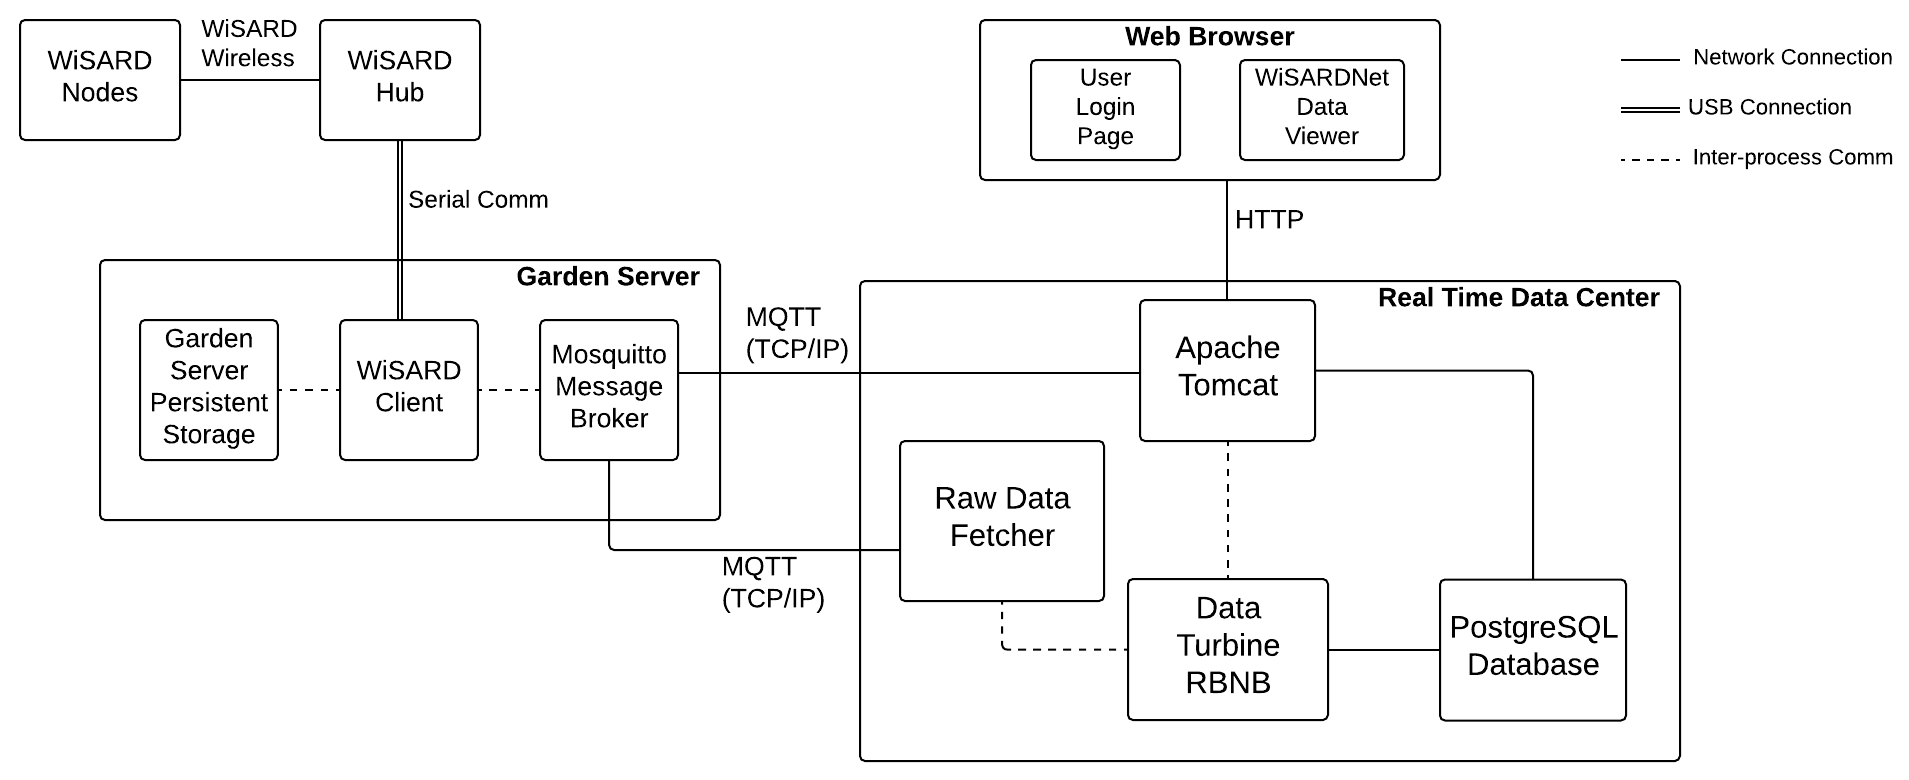
\includegraphics[width=\textwidth]{figures/wisardnet_ci_final}
	\caption{Cyberinfrastructure hardware and software component hierarchy}
	\label{fig:device_hierarchy}
\end{figure}

\section{WiSARD Nodes}
A Wireless Sensor/Actuator and Relay Device (WiSARD) is  modular, adapting easily to the different sensing and actuation needs of users. Flexibility and energy awareness are the two driving design motivations in the WiSARD development. At the heart of each WiSARD device is a central processor (CP) which governs the operation of the device and its peripherals. The CP dictates when and how tasks will be scheduled and executed, establishes and manages wireless links to other WiSARDs, facilitates the storage of sensor readings, and offloads the sensing and actuation tasks to daughterboards called satellite processors (SP). A WiSARD can accommodate up to four different SPs. This enables each WiSARD to perform a variety of tasks specifically tailored to meet the needs of researchers and experimenters. The modular design allows the CP to offload sensing operations to its SPs which can execute tasks in parallel with CP operation. 

Both CP and SP boards use a Texas Instruments MSP430 16-bit ultra-low-power microcontroller. This microcontroller has a variety of features and can be placed in various low-power modes. The low-power modes of operation, accompanied by energy-conscious software design, allow for a WiSARD to operate on a single pack of three AAA batteries for many weeks or even months, depending on the rate at which the devices dispatch their sampling operations. The CP also connects to a radio board which uses an Analog Devices ADF7020 RF transceiver module that operates in the 902-928 MHz license-free ISM band.  When WiSARDs are powered up, they autonomously form a self-organizing and self-healing multi-hop wireless ad-hoc network~\cite{Flikkema}. A special WiSARD which is assigned the software role of Hub acts as the base station, and is connected to an embedded Linux computer referred to as a garden server. 

\section{Middleware}

%The central architectural component which connects the garden servers to the RTDC is an open-source data streaming middleware software named Data Turbine. Data Turbine can be thought of as a data streaming engine acting as a ring-bufferred network bus (RBNB) which is a versatile and portable data streaming solution. Middleware software solutions operate under one of two operational paradigms: request/response or publish/subscribe. RBNB is a data broker which operates under the request/response paradigm of middleware software.  From an architectural standpoint, there are 3 core components to a Data Turbine implementation: servers, sources, and sinks. The Data Turbine server houses the actual data structure which manages the data and makes it available for request. Data Turbine Source objects aggregate data for insertion into the Data Turbine server. Alternatively, Data Turbine sink objects request data from the Data Turbine server and make it available to the process or user that desires it. Data turbine was written in Java, and is therefore versatile in the number of platforms upon which servers, sources, and sinks can execute. This, as well as the Data Turbine application programming interface (API) allows for a variety of data-centric applications and experiments to be performed. 

Middleware is a term which describes a software abstraction of the transfer of information from point A to  point B. By hiding the complexities of data transport behind a simple interface that connects two pieces of software, the development of powerful data processing and management tools can be accelerated. WiSARDNet relies heavily upon the use of middleware to make the WSN data available to the rest of the world. The central architectural component that connects the garden servers to the RTDC is MQTT. MQTT is a data transfer protocol created by IBM that utilizes the publish/subscribe middleware paradigm~\cite{HunTruSta08}.\\

In order for MQTT to be explained in the context of this work, a few more terms need to be defined. This work is concerned with the reconfiguration of WiSARD nodes. Each WiSARD is comprised of multiple devices. A device is a singular piece of hardware; a transducer, a CP, a SP, and a radio are each an example  of a device. The set of operational parameters that control a device is called a configuration. A deployment is an instance of a device and its configuration. Reconfiguration is the process of changing the operational parameters of one or more deployed devices.\\

MQTT facilitates the sharing of data between applications through the use of brokers. A broker is an application that sends and receives data to and from other applications. The transferred data are called messages. When a program sends a message to a broker, it labels the message with a topic name. The program sending the message is called a publishing client. Any program that is interested in data from a publishing client can subscribe to a topic through the broker; this is called a subscription client. All messages from publishing clients that are labeled with a matching topic will be sent by the broker to all subscription clients that have subscribed to that topic.\\

WiSARDNet uses Mosquitto~\cite{mosquitto}, an open source implementation of a message broker that uses the MQTT protocol. A message broker installed on each garden server keeps all of the data from that site in non-volatile memory. The data is organized into archive files at regular time intervals. To transfer the data from the WiSARDs to the broker, a Java application referred to as a WiSARD client uses MQTT messages to publish data. The RTDC can then retrieve the data using a subscription client that connects to the garden server message brokers over cellular or satellite connections.\\

An MQTT subscription client for each garden site runs at the RTDC and is responsible for subscribing to all the data published to each broker. These subscription clients are what is referred to in WiSARDNet as a raw data fetcher (RDF).  The purpose of the RDFs is to retrieve all of the data from all of the gardens so that the data is accessible for processing, storage, or viewing. These processes are discussed in detail in the following section.\\

%Within the WiSARDNet CI, each garden server runs a local instance of the Data Turbine server. Data Turbine Source objects are small software programs which funnel data gathered from the local WiSARD network feed data into the Data Turbine server. Alternatively, sink objects pull data out of the Data Turbine server. Data Turbine uses what is referred to as a channel map as a means to associate individual data channels with the Data Turbine streams that connect sources and sinks to the Data Turbine server. At the RTDC, a much larger instance of the Data Turbine server runs, with source objects connecting to each garden server. By initializing a Data Turbine sink, a user or application may request specifically identified data channels from the Data Turbine server using a channel map with the names defined by the user in the source. In the WiSARDNet CI, the Data Turbine server at the RTDC requests all new data at regular intervals from the Data Turbine server instances at each garden, and inserts the data into a single central location. These requests are made via TCP/IP connections between the garden servers and the RTDC via their cellular or satellite based Internet connections. The WiSARDs themselves are not directly ip-addressable and therefore funneling data to the RTDC via each garden's base station greatly simplifies the procedure of requesting data from each location.

\section{Real-time Data Center}
The RTDC is a collection of compute and data servers that host a Apache Tomcat web server, a Mosquitto MQTT subscription client, an instance of an open-source data streaming middleware called Data Turbine, a PostgreSQL relational database, and all of the data management processes and applications which interact with the WSN. The RTDC has several functions, the first of which is to retrieve all of the WSN data from each of the gardens. The RTDC is a centralized destination for all of the network's data streams. From this location, applications can access, store, and modify data for their various needs, as opposed to having to interact with multiple networks individually. For instance, a process which reads in raw data streams from temperature sensors might need to calculate human-readable values from the raw sensor readings. A single data converting processor which moves data from raw transducer values to human-readable values, can easily acquire all of the raw data streams for temperature sensors at all network locations with a single fetch, rather than requiring that the process fetch the raw data from each specific garden individually. Additionally, aggregating all data at the RTDC greatly simplifies archival and backup procedures.\\

Another function that the RTDC performs is the execution of applications and processes which interact with the WSNs and their data. One example of an application running on a server at the RTDC might be an experiment which attempts to maintain equal soil moisture readings at two different geographic locations. The RTDC servers possess high-performance computing hardware that many applications and processes can use to interact  with the networks in real-time.\\

\subsection{Relational Database}
Relational databases provide a flexible way to store and access large amounts of data. A relational database is composed of one or more tables; tables are 2 dimensional matrices of rows and columns. According to Rockoff ~\cite{rockoff2010language}, rows and columns are referred to as records and fields, respectively. An entry in a database table occupies a single row and each field corresponding to a different attribute of that entry constitutes a new column. For example, a table which stores people might have columns for an identification number, a name, an address, and a telephone number. An entry of a new person into this table would occupy a single row, with the data matching each of the attributes would occupy the rows' intersections with each column. Formally, these columns are referred to as primary keys, as they uniquely identify database records. The database at the RTDC has numerous tables which store information about every device, garden location, and sensor reading.\\ 

In WiSARDNet, data streams are archived in a PostgreSQL table. Other tables in this database store all of the meta-data and logistical information regarding all WSN devices, as well as every data point sampled from all transducers. Additionally, there are many data streams that need to be tracked and archived such as diagnostic and control data, error reporting, and other useful information. An example of diagnostic data might be the logging of a device restart event; such events can be crucial in detecting and analyzing network performance issues.\\

The PostgreSQL database where all of this data is archived is physically located on its own server hardware at the RTDC, separate from the other data management and processing clients. By placing the database on its own server hardware, the database has exclusive access to dedicated processing resources to allow for the quickest possible query and insert times.\\ 

\subsection{Data Schema}
WiSARD hardware components are subject to a design hierarchy that specifies how they interact. Figure \ref{fig:device_hierarchy_edit} shows the hierarchy of the WiSARD hardware components. 

\begin{figure}[H]
	\centering
	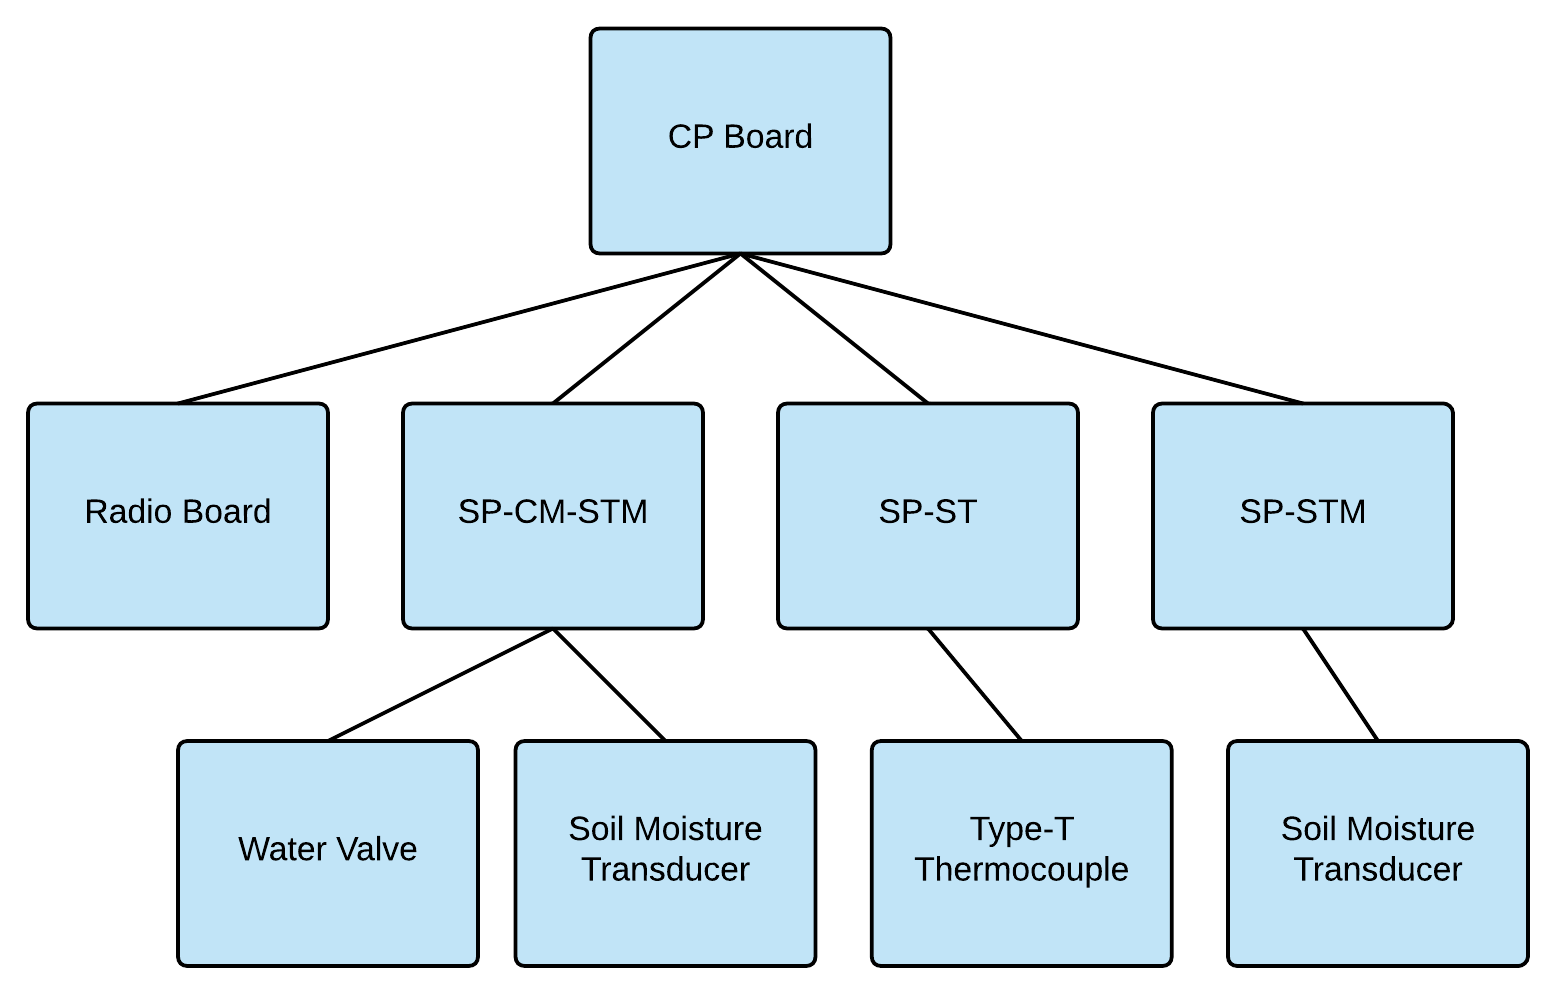
\includegraphics[width=\textwidth]{figures/wisard_device_hierarchy.png}
	\caption{Example of a WiSARD's device relationship structure. This WiSARD }
	\label{fig:device_hierarchy_edit}
\end{figure}

In a similar manner, the data gathered in WiSARDNet follows a design hierarchy that specifies how data is organized. The organizational structure of the the data tables and their relations, or the data schema as it is commonly referred to, was specifically designed to best accommodate changes to the configuration status of WiSARDNet devices. Every piece of hardware is referred to in the data schema as a device, and therefore the primary table in the data schema is the Device Table. A record in the Device Table will describe any device of any type. For instance, a radio, a soil-moisture transducer, a satellite processor, or a garden server are all devices that have a record in the Device Table. The configuration of a device might change at some point in time; it might be moved to another location, it might be upgraded or replaced, or it might receive a new firmware version. In this schema, the device's software parameters, hardware configuration, and state of operation are all encapsulated in a Deployment. Using the hierarchical structure of the WiSARD hardware, we use a tree structure in grouping devices together through their deployment records. Figure \ref{fig:deployment_hierarchy_edit} shows how devices and deployments are structured in the database. Each deployment record has a field for a parent device deployment. 

\begin{figure}[H]
	\centering
	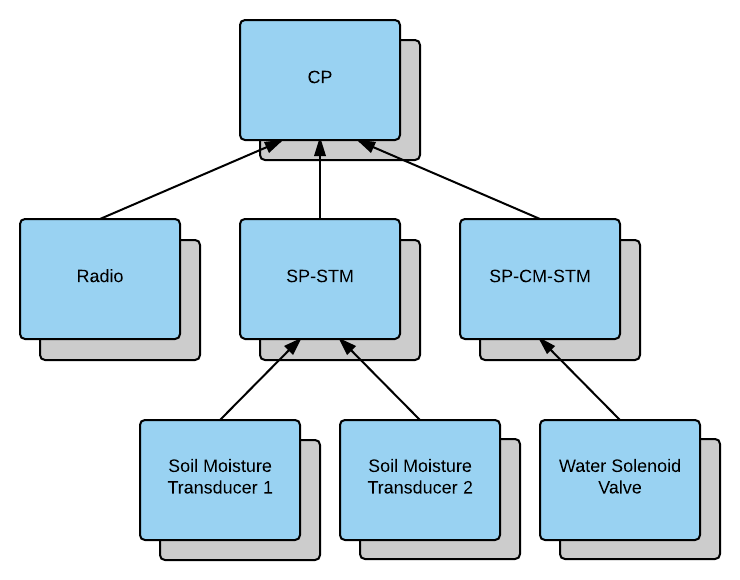
\includegraphics[width=\textwidth]{figures/deployment_hierarchy.png}
	\caption{A visual showing each device (background) and its active deployment (foreground) and how the deployments are connected}
	\label{fig:deployment_hierarchy_edit}
\end{figure}

When a transducer is attached to a satellite processor, then its active deployment record references the satellite processor's deployment record in the parent deployment field. These are recorded and tracked through the Deployment Table where each record is a particular deployment that references a device record in the device table. When a change is made to any of the parameters tracked in the deployment table, the device is considered as having a new deployment, and therefore a new record is inserted into the deployment table, and the device record is referenced by the new deployment. The key field in the deployment table is a binary field which stores a true/false value of whether or not the deployment is active. Once a deployment is changed, the old deployment becomes inactive and the new deployment becomes active. Over time, many deployment records may accumulate for a particular device as changes are made; the entire history of the device is stored so that for any given data point, the deployment configuration of the device associated with that data sample is accessible.\\

Having the ability to store and track each device's configuration and related meta-data in the database is of great value in the management of the networks and the various experiments. When a WiSARD is ready for deployment at a garden site, a deployment record is created with all of its configuration data, the deployment record is set to active, and the start date and time is set. As long as the device remains in this configuration, the deployment object pointing to that device will remain active. If a device is changed in any substantive way, the following actions are taken:

\begin{enumerate}
	\item The deployment record referencing the changed device is set to inactive.
	\item The current time is inserted into the stop-time field of the deployment record
	\item A new deployment record is inserted into the deployment table
	\item The parent field of the new deployment record references the deployment record of the parent device
	\item The active status field of the new deployment record is set to active
	\item The current time is inserted into the start-time field of the new deployment record
\end{enumerate}

By following this procedure, device configurations are easily accessible from the database. A previous deployment exists as a single record in the Deployment Table which is trivial with regards to computational complexity and storage resources. This approach is simple, intuitive, and scales well as the number of devices deployed in the field increase. With this paradigm, a data sample is not merely a sample from a device,  it is a sample from a specific deployment of a device. When a device's configuration is altered, a new deployment is created for that device and the data generated by that device references the new deployment record.\\

When new data from WiSARDs arrive at the RTDC from the MQTT broker, they need to be accessible for users and other services to request. Data Turbine's network accessible ring buffer data structure works well for this purpose. At the RTDC, the data streams arriving via MQTT are placed into Data Turbine's ring buffer in accordance with the stream name which identifies the device from which the sample was taken. Since the complexities of WiSARD configurations are handled via storing their configuration data in database tables, archival of sampled data in the database becomes a simple procedure. All samples from all streams are placed as individual records in a table named Data. In addition to the sampled value and the time that it was sampled, the value can be related to the specific device and deployment records via its Data Turbine stream name. In this way, data archival of acquired samples is extremely simple and all information regarding a device and its samples is easily accessible and intuitively obtained through the thoughtful design of the data schema. 

\section{Summary}
WiSARDNet is a WSN CI which was designed from the ground up to be modular, scalable, and accessible to users. The Mosquitto MQTT broker, the data streaming middleware Data Turbine, and the RTDC enable data sampled by sensors to be retrieved, managed, processed, and archived into a PostgreSQL database. The way in which WiSARD meta-data and configuration information is stored and accessed is critical for the development of a network configuration software which comprises the work of this thesis. How these features are utilized in the network management software is described in further detail in Chapter 4. % WSN Platform

% Chapter 4
\chapter{Network Reconfiguration Software} % Write in your own chapter title
\label{Chapter 4}
\lhead{} % Write in your own chapter title to set the page header

\section{Overview}
This chapter discusses the software developed in this thesis. First, this chapter discusses the procedures involved in network reconfiguration and the features required to achieve that goal. Next, the features are discussed in terms of the software functionality that needs to be implemented. Finally, the chapter discusses how the different functionality is grouped into software modules. The specifics of how each module works is described in Chapter 5.

\section{Approach}
To achieve network reconfiguration functionality within WiSARDNet, the following features are required: 

\begin{itemize}
	\item The user needs an up to date understanding of a WSN's configuration.
	\item The user needs to be able to specify the desired configurations or features they want to make to a set or subset of WSN nodes.
	\item Users need to be able to communicate configuration changes to the WSN. 
	\item The WSN needs to execute the new behaviors that the user specifies.
	\item The system needs protections that ensure continued and correct WSN operation.
\end{itemize} 

As was shown in Chapter 2, there are many ways that other WSN platforms have approached network reconfiguration. For the work in this thesis, a database abstraction is used as the general approach for structuring WSN reconfiguration. The specific abstraction used is that the WSNs in WiSARDNet can be viewed as a database of dynamic heterogeneous behaviors. By viewing the WSNs from a database perspective, queries and inserts become the language that users can use to interact with the WSN. The database paradigm simplifies the complexity of WiSARDNet and guides the design of WSN reconfiguration.

In addition to the database abstraction, another abstraction is used to approach WSN reconfiguration. As described in Chapter 3, the components that comprise a WiSARD are represented in the WiSARDNet PostgreSQL database as individual devices with deployments that describe their current state. Since a WiSARD is a collection of these physical devices, it is useful to represent the device deployments as WiSARD objects. This is especially true given the number of database relationships that are managed, such as those to parent deployments, device types, sites. Figure \ref{fig:wisard_object} shows an example of how a WiSARD encapsulates multiple related deployments. 

% wisard abstraction
\begin{figure}[H]
	\centering
	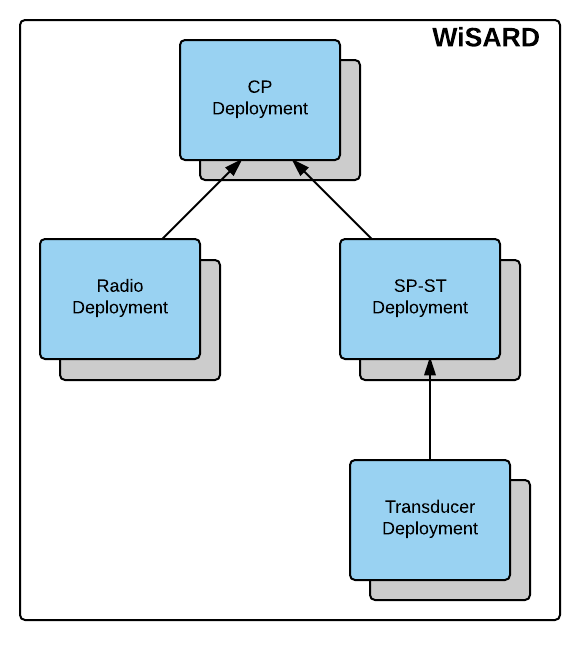
\includegraphics[width=.6\textwidth]{figures/wisard_abstraction_example.png}
	\caption{An example of the WiSARD abstraction used to encapsulate multiple related device deployments. Each arrow represents a deployment record's reference to its parent deployment.}
	\label{fig:wisard_object}
\end{figure}

% wisard database representation
\begin{figure}[H]
	\centering
	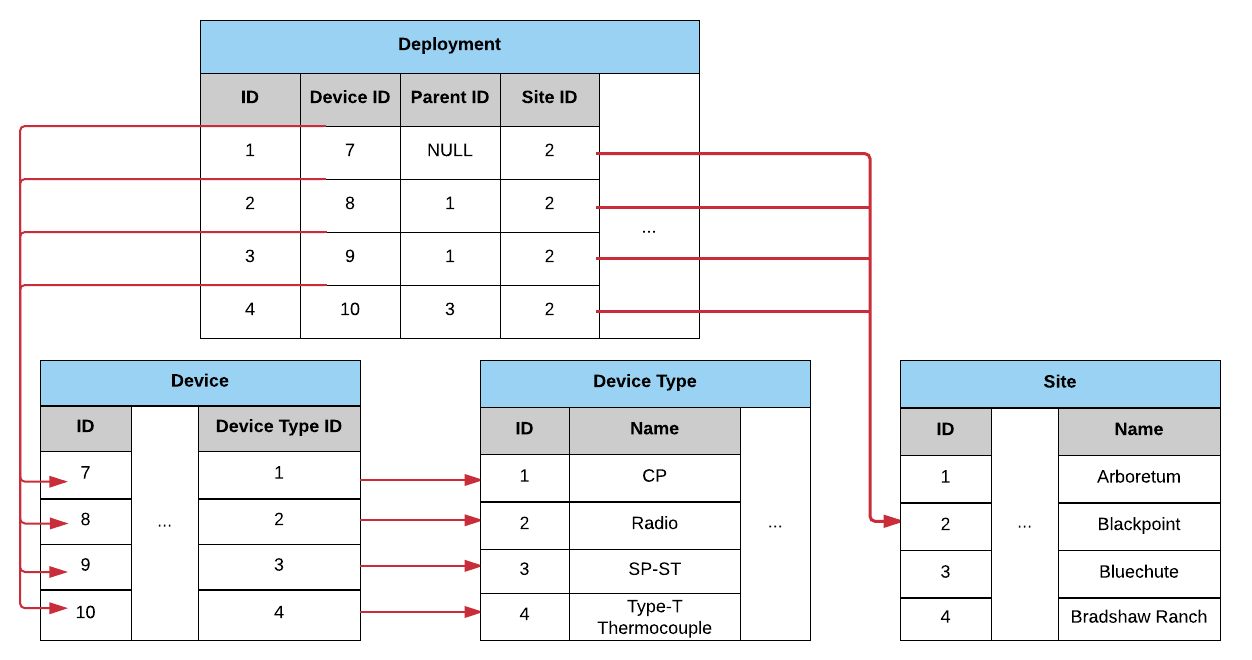
\includegraphics[width=\textwidth]{figures/wisard_abstraction_example_database.png}
	\caption{Database representation of example WiSARD abstraction from Figure \ref{fig:wisard_object}. The arrows illustrate foreign key references between records in different tables.}
	\label{fig:wisard_object_database}
\end{figure}

Using WiSARD objects to encapsulate multiple related device deployments means that a WSN can be reconfigured by updating sets of WiSARDs rather than many individual deployments. The database abstraction of the WSNs and the WiSARD abstraction of the WSN node devices together provide the conceptual foundation for the reconfiguration features to be implemented in software. The WiSARD abstraction is implemented in code as a Java class. Each instance of the WiSARD class encapsulates all of the device deployments of a WiSARD object as shown in Figure \ref{fig:wisard_object}. Instances of the WiSARD class provide methods for accessing records referenced by deployment foreign keys, similar to navigation properties in Object Relational Mapping (ORM) objects. For example, devices in a WSN are deployed at locations where a researcher would like to gather data. A Site database table was created in order to store information related to such deployment locations. One of the ORM-like methods that a WiSARD object provides is one that will return the Site record referenced by the WiSARD deployments. In addition to the WiSARD class, there are classes for encapsulating other tables in the database, including the Site Table. When a WiSARD returns a deployment's Site record, it is in the form of an instance of the Site class. The database tables and their related Java classes are discussed in further detail in the following Section. 

%%%%%  FINISH THIS SECTION  %%%%

\section{Solution Description}
Implementing WSN reconfiguration functionality into an existing software system requires that new code modules be developed that account for all of the known use cases and as many future use cases as possible. A practical example is a scenario where a researcher wants all soil moisture transducers attached to WSN nodes in a specific region to be sampled at twice their current sampling rate. Performing this procedure involves the user specifying the region and sensor types needed to produce a matching set of WSN nodes, and that he/she wants the sampling rate of those transducers to be changed. The software needs to validate that there are no conflicts between that user's requested changes and the existing operational configurations of the node. Finally, the nodes will each be signaled via command packets, execute the specified change in configuration, and will then alert the user of the changes made.

\subsection{Implementing Functionality}
Each of the features described in the previous section needs to be implemented as software functionality to be used in the WiSARDNet system. This section describes the software tasks for each feature. 

\subsubsection{Identification of WSN Nodes}
Transducer samples, sensor types, WiSARD role information, and hardware metadata are all stored in database tables and are necessary to determine which nodes will need to be reconfigured. The first stage in reconfiguring a WSN is the specification of the node or nodes whose configurations will be modified. This operation begins with a user specifying search criteria for a set of WiSARD that they want to reconfigure. Next, static and dynamic WiSARD information is gathered by querying a set of PostgreSQL database tables that have all of the information that describes a WiSARD. Table \ref{tab:db_tables} shows all of the tables that are queried when searching for WiSARDs and describes the information stored in each table. The results of these queries are then stored in instances of Java objects created for each table.

%%% FIX TABLE REFERENCE %%%

%%% ADD TABLE OF DATABASE TABLES %%%
\begin{table}[H]
	\centering
	\renewcommand{\arraystretch}{1.1}
	\begin{tabu}{|X[2.5,c]|X[8,c]|}
	\hline
	\textbf{Database Table} & \textbf{Description}\\
	\hline
	Device & Stores a record for each device in WiSARDNet\\
	\hline
	Deployment & Stores a record for each deployment of a device\\
	\hline
	DeviceType & Stores a record for each possible type of device\\
	\hline
	DeploymentType & Stores a record for each type of deployment \\
	\hline
	Site & Stores geographic information about each garden site\\
	\hline
	Experiment & Stores a record for each WiSARDNet experiment\\
	\hline
	\end{tabu}
	\caption{A list of the database tables containing information about WiSARDs and their configurations.}
	\label{tab:db_tables}
\end{table}

The next step in this procedure is to filter all of the queried information against the search criteria that a user has specified. Once a list of WiSARDs that match the search criteria is obtained, the user can specify a new configuration to be applied to each WiSARD in that list. The software which obtains search criteria, translates information from  database tables to Java objects, and filters WiSARDs is described in further detail in the Chapter 5.

\subsubsection{Describing the New Configuration}
A WiSARD's task execution is governed by a set of configuration parameters stored within the device's non-volatile memory; this area of memory is called the task control block. Changing a device's behavior is achieved by overwriting specific values within the task control block with values that represent different behaviors. The user must describe the changes to the system so that the correct fields in the task control block can be overwritten with appropriate values corresponding to the new behaviors. This is achieved by encoding different behavior or behavior profiles into control sequences which the WiSARDs are able to decipher. 

\subsubsection{Validating the New Configuration}
As the number of configuration changes and the number of affected WSN nodes increases, the possibility of errors or resource conflicts between experiments also increases. To prevent conflicts, there is a need to validate that the intended changes will not interfere with other experiments each node is associated with. This is achieved with user access control and command validation.

User access control is the process of restricting the access of users to specific pieces of hardware or software based on a set of rules and permissions that govern the extent to which they can interact with the WSN. For example, a researcher should not be allowed to reconfigure another researcher's hardware or reconfigure the WSN in a way that will adversely affect other experiments. User access control in WiSARDNet is achieved by using database tables to store information about users and the WiSARDs they are allowed to change.

Command validation is the process of analyzing the configuration changes a user intends to make to a specified set of WiSARDs and determining whether the change is feasible and safe to make. For example, a user should not be allowed to send a command that will cause a WiSARD to misbehave or prevent it from performing its essential duties. Both user access control and command validation are essential in validating a configuration before execution.

%%% ESSENTIAL DUTIES? %%%

\subsubsection{Command Synthesis}
Once the user has specified a new configuration, command packets are automatically generated. A command packet is a structure which contains a control sequence, configuration parameters, and network routing information which will allow each command to be sent to its intended WiSARD. The control sequences are defined by software classes, the command parameters are obtained from the user's configuration specifications, and the routing information is obtained from the list of WiSARD objects. Once generated, the command packets are added to MQTT messages and flushed from an MQTT publisher client at the RTDC to the MQTT broker at the destination garden server. Each garden server has a WiSARD client which retrieves command packets from the local MQTT broker and sends them into the WSN via the hub node. 

\subsubsection{Executing the Reconfiguration}
When a WiSARD receives a command message from a parent node, the WiSARD parses the command message and schedules a task to execute the command. When a WiSARD executes a command, a report message is created and sent back through the network to the RTDC. The report message will confirm that the task was successfully executed or report that it failed if the task did not execute successfully.

\subsubsection{Verifying the New Configuration}
All data generated by a WSN is sent to the RTDC in the form of data streams. Each transducer reports its samples as specific streams defined by the device relationship structure discussed in Chapter 3. A WiSARD also reports diagnostic and error information as data streams in the same manner. After making a configuration change, a WiSARD reports its new configuration through a designated data stream to the RTDC. 

%%% ADD MORE TO THIS LATER %%%

% software modules - WiSARD Browser, Command Generator, Validation
\subsection{Software Modules}
The software implementation of the functionality described in the previous section is grouped into three distinct modules:

\begin{itemize}
	\item Wisard\_Browser\_Module
	\item Cmd\_Generation\_Module
	\item Validation\_Module
\end{itemize}

Wisard\_Browser\_Module contains the functionality that can identify sets of WiSARDs that match a user's search criteria. Additionally, this module is responsible for providing an up to date view of a WSN. The functionality which allows a user to describe a new WSN configuration and signal those changes to the WSN is grouped into Cmd\_Generation\_Module. The functionality which validates the safety of a new configurations, checks for conflicts, and implements user access control into the system is grouped into Validation\_Module. Figure \ref{fig:wisardnet_ci_additions} illustrates the new modules added to the WiSARDNet CI, as well as the existing software systems with which they communicate.

% wisardnet ci additions
\begin{figure}[H]
	\centering
	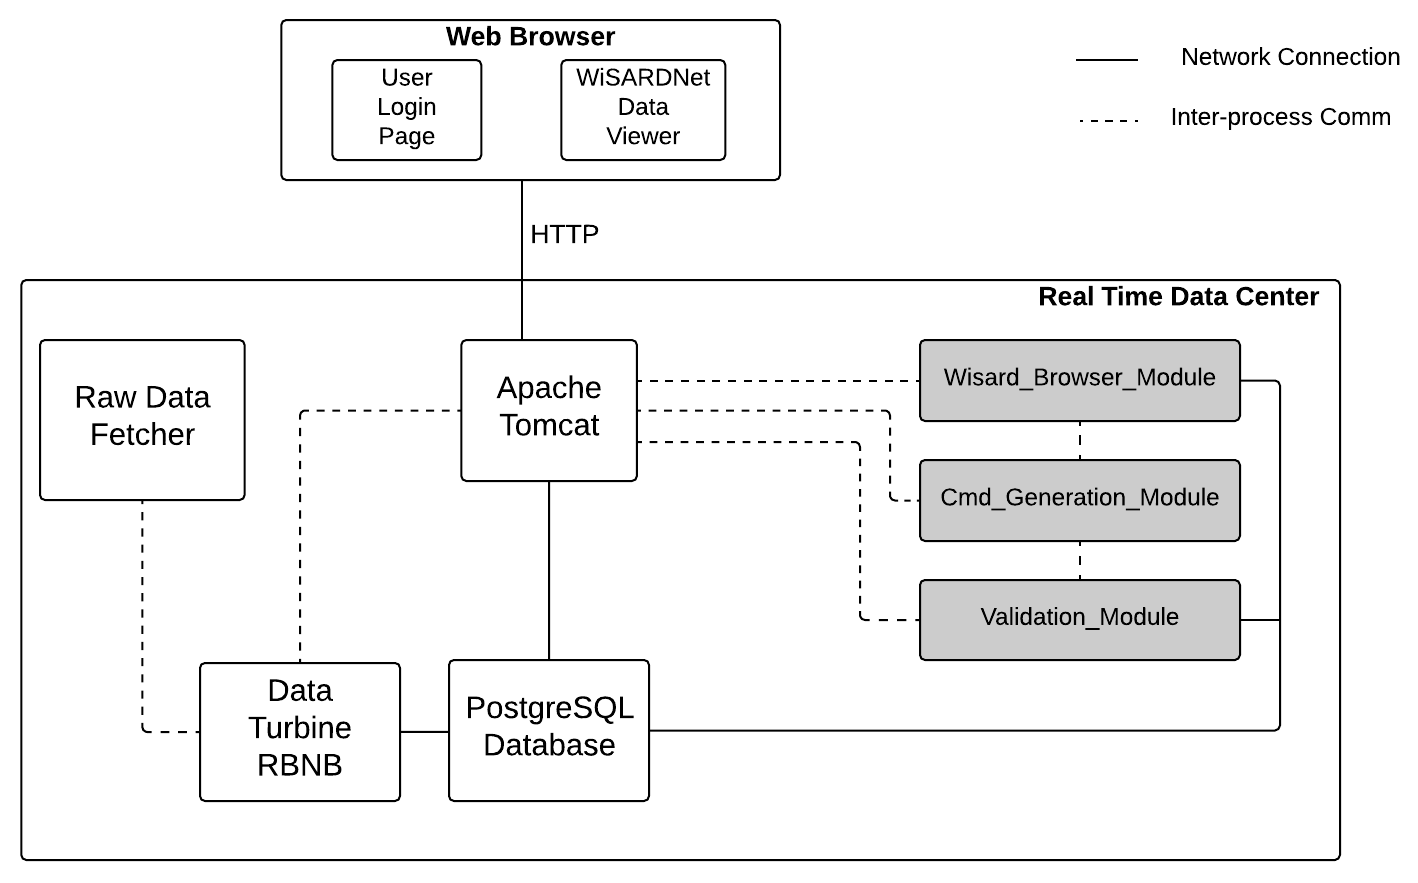
\includegraphics[width=\textwidth]{figures/wisardnet_added_modules.png}
	\caption{The software modules being added to the WiSARDNet cyberinfrastructure for WiSARD reconfiguration are shown in the shaded boxes. }
	\label{fig:wisardnet_ci_additions}
\end{figure}

Each software module contains separate functionality, but they interact and share information with each other as well as the other components of WiSARDNet. Wisard\_Browser\_Module interacts with the web portal user interface, it gathers information about the WSN nodes from the PostgreSQL database, and provides sets of WiSARDs to the other modules. Cmd\_Generation\_Module interacts with the WiSARDNet web portal to generate commands based on a user's input. Additionally, it accesses the list of WiSARDs that Wisard\_Browser\_Module produces. This module accesses the PostgreSQL database to enable stored behaviors to be turned into commands. Lastly, this module provides information to Validation\_Module so that the commands can be verified. Validation\_Module gets session variables from the web portal to authenticate users. It also takes in a set of commands from Cmd\_Generation\_Module, that can validate and report its results.  To verify that the user is permitted to run a specified command, the user and command need to be compared against permission records stored in PostgreSQL database tables. These tables are discussed in detail in Chapter 5.

In summary, the functionality is grouped into three distinct software modules: Wisard\_Browser\_Module, Cmd\_Generation\_Module, and Validation\_Module. These modules need to be able to interact with the different components of the WiSARDNet CI as well as with each other. The software implementations of the modules are discussed in Chapter 5. % Modeling

%% Chapter 5

\chapter{Software Module Implementation}
\label{Chapter 5}
\lhead{}

% use \verb|Samp_Dist_Corr| notation for underscores
%\documentclass{article}
%\texttt{Samp\_Dist\_Corr}
%\verb|Samp_Dist_Corr|
%\texttt{Samp\char`_Dist\char`_Corr}

\section{Overview}
This chapter explains how each of the three modules discussed in the previous chapter are implemented in software. First, Wisard\_Browser\_Module is discussed. Cmd\_Generator\_Module is discussed next, followed by Validation\_Module. Validation\_Module is discussed last because it has the broadest impact on the other modules and the system as a whole. 

\section{WiSARD Browser}
Wisard\_Browser\_Module is a collection of software components which address four major objectives.

\begin{itemize}
	\item Allow a user to specify WiSARD search parameters through a user interface
	\item Search the WiSARDNet PostgreSQLdatabase for WSN state information
	\item Produce a set of WiSARD data objects matching the search criteria specified by the user
	\item The module should integrate with the existing WiSARDNet software
\end{itemize}

% flow of execution - wisard browser module
Figure \ref{fig:wisard_browser_flow} shows the flow of execution for this module. Each procedure shown is described in this chapter.

\begin{figure}[H]
	\centering
	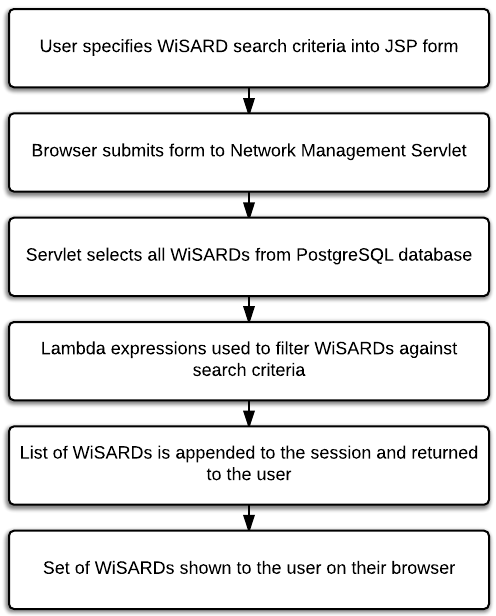
\includegraphics[width=0.6\textwidth]{figures/flow_diagram_wisard_browser.png}
	\caption{A flow diagram showing the actions performed by Wisard\_Browser\_Module to obtain a list of WiSARDs based on user specified search criteria.}
	\label{fig:wisard_browser_flow}
\end{figure}

\subsection{Obtaining the User's Search Criteria}
A user of this system needs an interface that allows them to send and receive information to Wisard\_Browser\_Module, Cmd\_Generation\_Module, and Validation\_Module. To create this interface, JSP (JavaServer Pages) and Java servlet technologies are both used. A JSP page presents information to a user through a web browser and gathers user input necessary for back-end operations. The JSP page sends information to and from a servlet called NetworkManagementServlet, which is a java class that implements methods that respond to Get and Post requests from a web browser. Because NetworkManagementServlet is an instance of a Java class, it has the ability to interact with instances of other classes. JSP/servlet interaction is the communication pipeline which allows the user to interact with these three software modules. Figure \ref{fig:jsp_interaction} illustrates how NetworkManagementServlet is used to send and receive information between a user's browser to the appropriate software module. 

\begin{figure}[H]
	\centering
	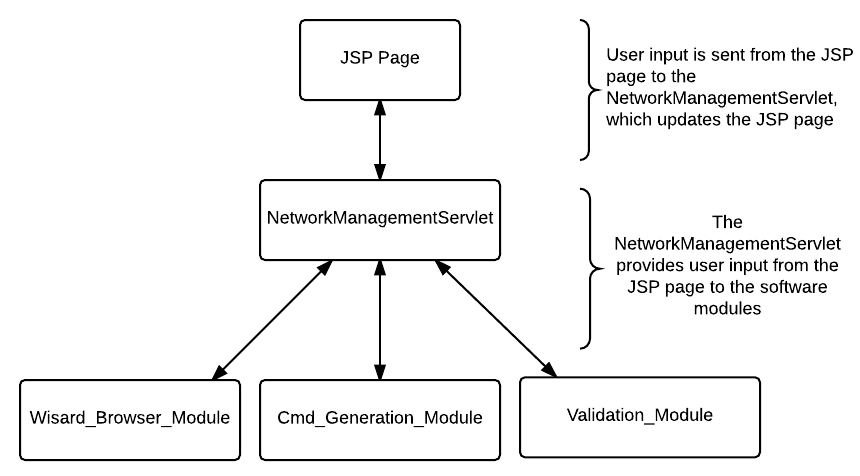
\includegraphics[width=\textwidth]{figures/jsp_interaction.png}
	\caption{NetworkManagementServlet relays information between the user interface and Wisard\_Browser\_Module, Cmd\_Generation\_Module, and Validation\_Module.}
	\label{fig:jsp_interaction}
\end{figure} 

A JSP web page provides a simple interface for the user to populate an HTML form. The attributes that can be used to select a set of WiSARDs are (\ref{fig:jsp_ui_select})

\begin{itemize}
	\item WiSARD Network ID
	\item Device Serial ID
	\item Garden Site
	\item Associated Experiment
	\item SP type
	\item Transducer type
	\item WiSARD role
	\item Deployment Type
\end{itemize} 

\begin{figure}[H]
	\centering
	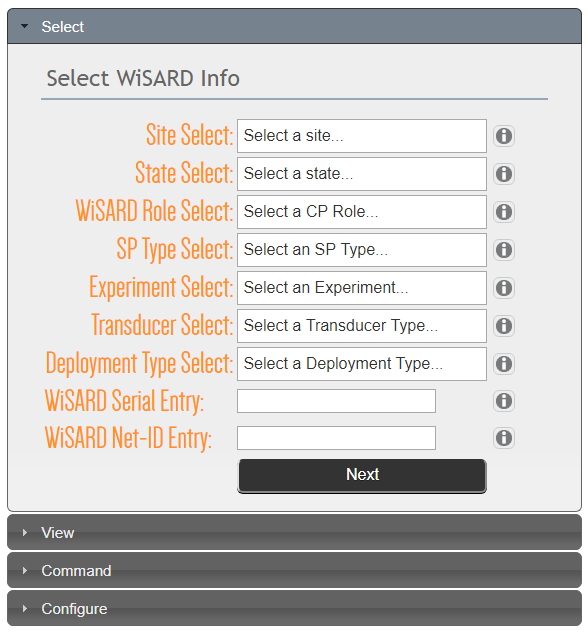
\includegraphics[width=0.6\textwidth]{figures/jsp_ui_select.png}
	\caption{A screen capture of the user interface page where a user specifies WiSARD search criteria. Wisard\_Browser\_Module queries the PostgreSQL database and creates WiSARD objects. The objects are then filtered against these search criteria to obtain a selection of WiSARD objects for a user to reconfigure.}
	\label{fig:jsp_ui_select}
\end{figure}

These attributes are are static or dynamic pieces of information that together represent the current state of the WSN nodes. Traditionally, this information can be obtained from a database query that can be written into a function or a method. Researchers and other users of WiSARDNet often have changing or new experiment requirements. It is important for the this software to be flexible and support changes to the WiSARDs and their configuration information. For example, if new WiSARD features are added, resulting in new fields in a database table or entirely new tables, the new features should not prompt extensive modification of the existing code. A new field or table would simply translate into new member variables in the WiSARD class. 

To implement the querying functionality for Wisard\_Browser\_Module that was discussed in 4.3.1.1, there were two possible design alternatives for the filtration that would result in a list of WiSARDs: PostgreSQL or Wisard\_Browser\_Module application code. PostgreSQL supports a wide variety of query features that enable sophisticated data processing and filtration of queried data sets. If achieving the fastest possible query speed was of great importance for this module, then all of the searching and filtration of WiSARDs from the user's search criteria should be handled by complex PostgreSQL queries. While query time is important, the benefits that can be gained at the sacrifice of processing speed make the other alternative desirable. Chapter 2 briefly explained some of the ways in which modern software development techniques such as behavioral parameterization can add functionality to software. For Wisard\_Browser\_Module, a functional data processing approach allows for development flexibility at the expense of performance overhead. This does not impact the performance of the system in a significant way because the amount of WiSARD deployment configuration information compared to the total amount of data stored in the database is trivial.

WiSARD objects translate from fields in database tables to software entities through the use of intermediate Java classes. A Java class with member variables that correspond to the different attributes that define a WiSARD's configuration, and methods to translate higher-level queries into database queries and results provides a foundation for objects to be created and passed from module to module. To achieve the desired flexibility, Wisard\_Broswer\_Module performs a single fetch to the database and retrieves all of the state information for all of the WiSARDs. It then formats the information from the query into member variables of WiSARD objects before adding them to a list data structure. All of this functionality is built into WiSARD class methods.

Once NetworkManagementServlet has obtained a list of all WiSARD objects, it then filters that list against the attributes which the user specified in his/her form submission. Utilizing functional data processing techniques supported by lambda expressions in Java 8, obtaining a list that matches a user's search criteria is simple and flexible. Below is an example of the way in which lambda expressions are used in this software to produce powerful results with a very small amount of code.

\begin{lstlisting}
return wisards.where((Wisard w) -> ''Arboretum''.equals(w.getSite()));
\end{lstlisting}

This statement returns an ArrayList named \verb|wisards| that contains WiSARD objects. The \verb|where()| method iterates over every entry in the ArrayList and only returns those not filtered out against the logic in the lambda expression. The lambda expression in this example compares the WiSARD site against a string containing the site name \verb|Arboretum|. Any WiSARD in the ArrayList that does not have \verb|Arboretum| as its site name will not be added to the returned ArrayList.

With one line of code, a data structure of WiSARD objects can  be filtered based on its member variables that would otherwise have required a specific database query. Additionally, values can be added to the same expression to create more complex data filtration without requiring that the underlying functionality be altered. This functionality provides a quick and versatile way to support changing project requirements for managing networks of WiSARDs without being restricted by specific database queries.

When a list of WiSARDs has been filtered to match a user's search, NetworkManagementServlet appends it to the session as a variable where it is accessible to the JSP page at the user's browser. The JSP page displays the WiSARDs and their deployment information for the user. From this point a user can decide to continue with reconfiguring the WiSARDs that this search has returned, or return to the form and specify a different set of WiSARDs. Should the user choose to continue on with the set of WiSARDs they have selected, the data structure is accessible within the browser session, ready to send to Command\_Generation\_Module.

\section{Command Generation}
Cmd\_Generation\_Module and Wisard\_Browser\_Module, are similar in that they both rely on user input being sent from the user interface to NetworkManagementServlet. The user will utilize the same JSP page's user interface as Wisard\_Browser\_Module to specify the change he/she would like to apply to the selected WiSARDs (Figure \ref{fig:jsp_ui_cmd}). Each menu option corresponds to a different configuration change that can be selected.\\

\begin{figure}[H]
	\centering
	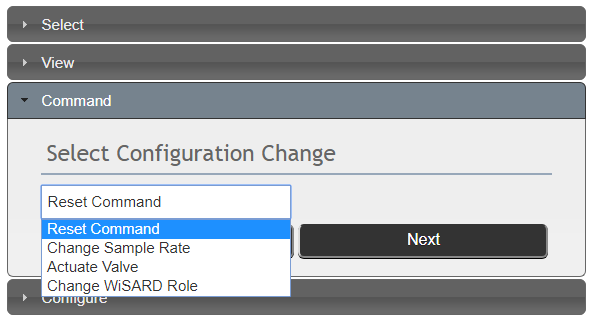
\includegraphics[width=0.6\textwidth]{figures/jsp_ui_cmd.png}
	\caption{A screen capture of the user interface that allows a reconfiguration command to be chosen. Once one is selected, Cmd\_Generation\_Module creates command objects for each WiSARD selected by the user. Each command object synthesizes a command packet that will produce the desired reconfiguration.}
	\label{fig:jsp_ui_cmd}
\end{figure}

Once a user has selected an option, the process of synthesizing the appropriate commands can proceed. Figure \ref{fig:flow_cmd_generator} shows the flow of execution for this module. Each procedure shown in the diagram is described in this section.\\

% flow of execution, cmd module
\begin{figure}[H]
	\centering
	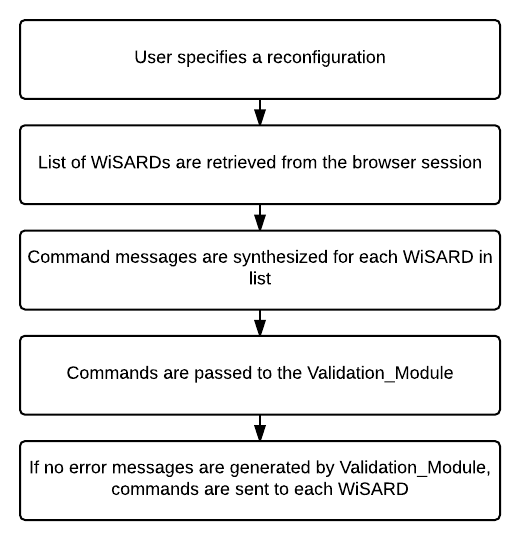
\includegraphics[width=0.6\textwidth]{figures/flow_diagram_cmd_module.png}
	\caption{A flow diagram showing each procedure Cmd\_Generation\_Module makes to synthesize WiSARD command packets that will perform a user specified reconfiguration.}
	\label{fig:flow_cmd_generator}
\end{figure}

To perform a reconfiguration in WiSARDNet, a specific command is generated and sent to each WiSARD that the change will affect. A command in the WiSARDNet communication protocol consists of multiple components. A hub address and a destination address describe which WSN the command should go to, and which WiSARD in the WSN that the command is intended for.

These potential reconfigurations include a soft reset on the device, updating a sampling rate, changing a software role or ID, or actuating a water valve. The list of commands that are possible with a WiSARD continues to grow with each new experiment and feature that WiSARDNet supports. For this reason, the of the design of command synthesis is implemented in a way that provides flexibility for future developments. In WiSARDNet, a command consists of a payload, an expiration, and a checksum. The payload is the byte stream which contains the command and its parameters the WiSARD will interpret and execute. The expiration is a value which the sender sets to prevent out of date commands from being executed. For example, if a command for some reason takes an hour to traverse the network, it may no longer be relevant and should not be executed. The checksum allows the destination WiSARD to verify that it received the command correctly. Each of these command components are encapsulated within a command class named NetManagementCommand.

The class definition for NetManagementCommand provides the member variables and methods for every command type. However, certain commands need additional parameters which aren't provided in NetManagementCommand's class definition. For this reason, a specific class is defined for each command type. Each command class uses inheritance to extend the member variables and methods provided by NetManagementCommand. Table \ref{tab:commands} lists each of the command classes that have been implemented and the reconfiguration change that they make.\\

%%% LIST COMMAND CLASSES HERE IN A TABLE %%%
\begin{table}[H]
	\centering
	\renewcommand{\arraystretch}{1.1}
	\begin{tabular}{|p{3cm}|p{11cm}|}
	\hline
	Command Class & Operation\\
	\hline
	SetSamplingRate & Adjusts the sampling rate of all transducers of a given type on a WiSARD\\
	\hline
	ResetCommand & Performs a soft reset on a WiSARD\\
	\hline
	ActuateValve & Actuates a latching solenoid water valve to an open or closed state\\
	\hline
	ChangeRole & Changes the software role of a WiSARD \\
	\hline
	\end{tabular}
	\caption{A list of each of the command classes that have been implemented.}
	\label{tab:commands}
\end{table}

To perform a reconfiguration, a command object is instantiated from the command class definition that corresponds to the user's specified configuration. The change that the user specifies will be enacted for all of the WiSARDs in the list that was added to the session by NetworkManagementServlet. Cmd\_Generation\_Module loops through each WiSARD and chooses the correct command parameters to include in the payload. Once the command objects have been successfully generated they are sent to Validation\_Module in a data structure, similar to the way that Wisard\_Browser\_Module provides the WiSARD list to Cmd\_Generation\_Module.


% 5.3 Command Validation
% 5.3.1 overview of validation
% - types of validation, UAC and safety
% 5.3.2 Permissions and UAC
% - Describe the design of permissions in the database
% - Remember that this will only be for WiSARDs now but state that the permission resource table could be expanded to anything 
% 5.3.3 Safety Validation
% - Describe use cases and how different commands require different checks
% - Describe design of commands with own validation logic so can be flexible
% - Describe that the validate method is given the database wisard and so all relevant parameters can be obtained through normal database relations?

\section{Validation}
Before commands can be sent out to reconfigure WiSARDs, there are two sets of checks which the commands must pass. First, Validation\_Module confirms that the user that submitted the commands has appropriate permissions to reconfigure the selected WiSARD nodes. Second, the module assess the commands for their impact on the system, and ensures that none of the changes will cause a WiSARD to misbehave. WiSARDs may have hardware that is shared between multiple experiments, and reconfiguring that WiSARD could have adverse effects on one or more experiments. The procedures that this module performs are shown in Figure \ref{fig:flow_validation_module}. Each of these procedures is described in this section.\\

% flow of execution, validation module
\begin{figure}[H]
	\centering
	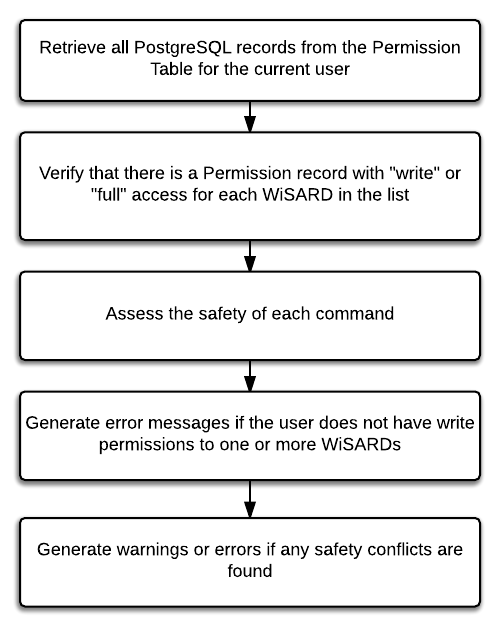
\includegraphics[width=0.6\textwidth]{figures/flow_diagram_validation_module.png}
	\caption{A flow diagram showing each procedure taken by the Validation\_Module to validate commands and user access prior to the reconfiguration of WiSARDs.}
	\label{fig:flow_validation_module}
\end{figure}

\subsection{Permissions and User Access Control}
The PostgreSQL database schema prior to this thesis had certain tables which could have been used for user access control, but the schema was not robust. To implement user access control in a flexible way, a better approach was needed. Two core abstractions of the existing database schema are used to design the permissions system for WiSARDNet. The first abstraction is that anyone to whom a permission might be granted is considered a permission entity. The second abstraction is that anything which would need its access restricted is to be considered a permission resource. After applying these two abstractions to the database, the Person and Organization tables are defined as permission entities. Likewise, the Deployment, Site, and Experiment tables are defined as deployment resources. With these two abstractions, granting permission simply becomes a mapping between a permission entity and a permission resource with a value designating the level of access the entity has to the resource.

Two access levels are used to denote permissions to resources: read and write. Table \ref{tab:permissions} describes what each permission level allows. Note that an entity with write access can override changes made by other entities with write access, but a warning message is generated to inform the user of the scenario. In this case, the user should proceed at their own discretion, and the permissions should be granted by an administrator with this in mind. In the greater context of the user access control paradigm, additional access levels could be added to allow delete privileges. Even though that use case doesn't directly correlate to the reconfiguration software, the paradigm still supports that feature for other applications. These two permission levels are sufficient to regulate how users  interact with the WiSARDs. 

This approach to user access control also provides a flexible way to manage other hardware or software resources which might be incorporated into WiSARDNet in the future. If a new type of resource is added to the system which is described by a new table, then adding a foreign key constraint from PermissionResource to the new table is all that is needed for a record in Permission to grant permissions to that new PermissionResource.\\

%\begin{table}[H]
%	\centering
%	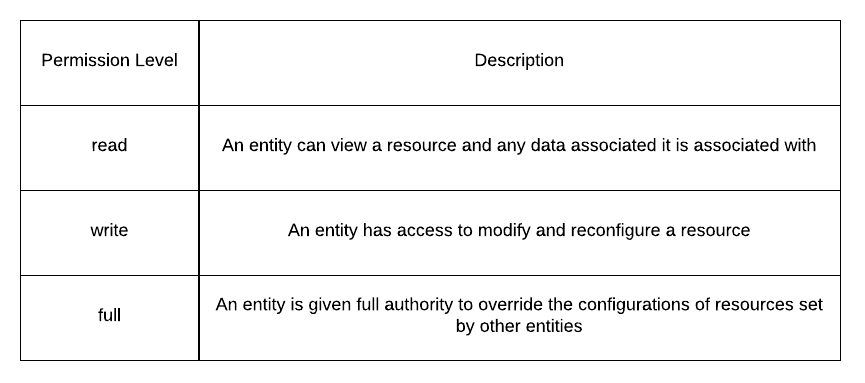
\includegraphics[width=\textwidth]{figures/permission_table.png}
%	\caption{A description of each access level an entity can be granted to a resource}
%	\label{tab:permissions}
%\end{table}

\begin{table}[H]
	\centering
	\renewcommand{\arraystretch}{1.1}
	\begin{tabular}{|p{3cm}|p{11cm}|}
	\hline
	Permission Level & Description\\
	\hline
	read & An entity can view a resource and all information regarding its deployment configuration \\
	\hline
	write & An entity has access to  modify and reconfigure a resource\\
	\hline
	\end{tabular}
	\caption{A description of each access level an entity can be granted to a resource.}
	\label{tab:permissions}
\end{table}

To implement user access control with this approach, three tables were added to the database. First, a table called PermissionEntity was created to reference the Person and Organization tables. Next, a table called PermissionResource was created to reference the Deployment, Experiment, and Site tables. Lastly, a table called Permission was created with foreign key constraints that reference the PermissionEntity and PermissionResource primary keys. Each record in Permission specifies an access level value that a PermissionEntity record has to a PermissionResource record. Figure \ref{fig:uac_simplified} shows these tables and their foreign key constraints. Each foreign key constraint references the primary key of the table that the arrow points to. The unnamed table on the right shows how the schema can be used to manage new resources in the future.

\begin{figure}[H]
	\centering
	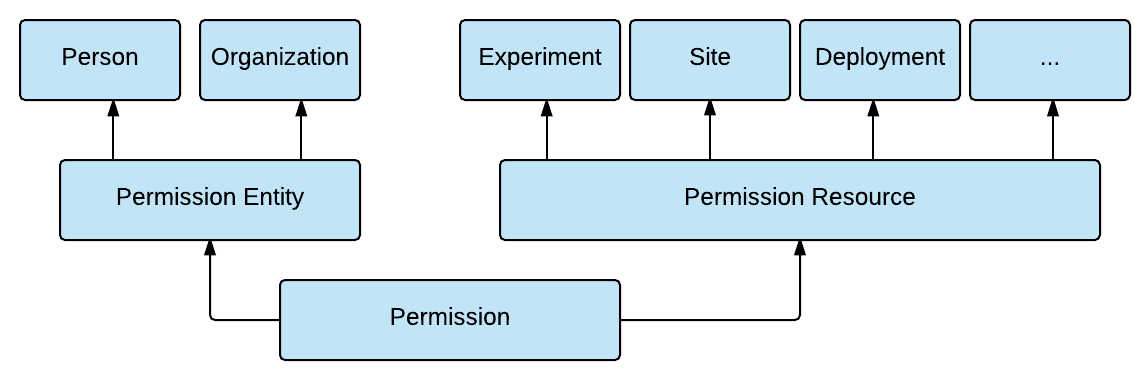
\includegraphics[width=\textwidth]{figures/uac_simplified.png}
	\caption{A diagram that shows how the three new permission tables are used to create a user access control schema.}
	\label{fig:uac_simplified}
\end{figure}

When Validation\_Module receives a data structure of command objects from the command generation module, the software in Validation\_Module first checks that there are no user access violations in any of the commands. This is done by iterating over each command object and performing a lookup to the permission table. The objective is to gather all of the Permission records whose permission entity matches the user that created the commands, and verify that a permission resource with write access is present, for the WiSARD in question. If the user is found to have insufficient permissions to execute a command, an error message is generated and added to a queue of messages that is displayed once Validation\_Module has iterated over every command. All commands with insufficient permissions are rejected, and will not be sent to the WiSARDs.

The validation logic for the reconfiguration software currently grants permissions to WiSARDs. However, the database schema supports a more granular level of detail. A record in the permission resource table could reference the deployment of a device, meaning that access to a WiSARD could be restricted down to individual transducers. 

\subsection{Safety Validation}
 If all of the commands pass the user access permission checks, then the module performs a configuration safety test on each command. The difficulty of the safety check comes from the different types of commands that can be executed, and the diversity of experiments and their needs. It is for this reason that the command class was designed such that each command type will implement its own safety logic. This way, when a new command is developed, the designer can build in a method which will perform a safety check within the context of that method. Figure \ref{fig:cmd_classes} shows the structure of these command classes and how they inherit and override behaviors.
 
\begin{figure}[H]
	\centering
	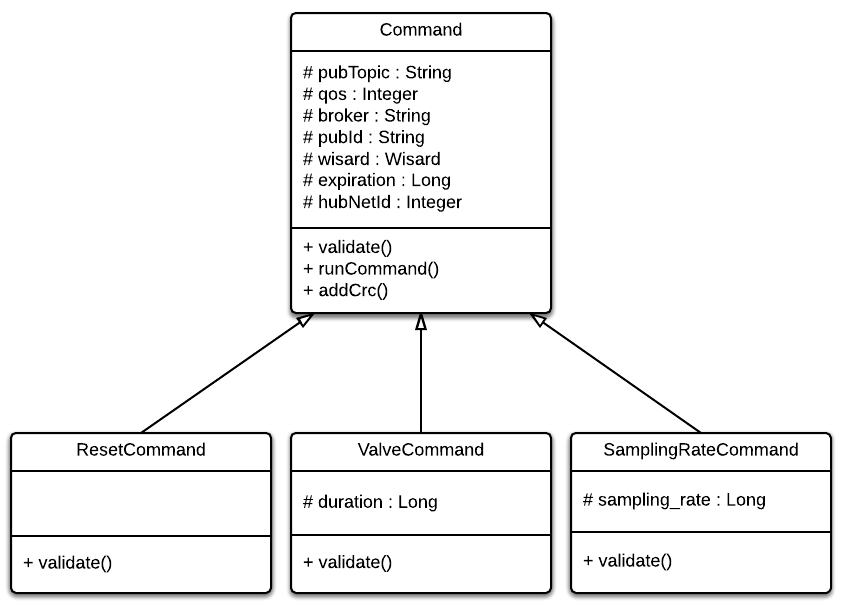
\includegraphics[width=\textwidth]{figures/command_class_diagram.png}
	\caption{A class diagram showing how new commands inherit from their parent class, yet implement their own validate method}
	\label{fig:cmd_classes}
\end{figure}
 
 A practical example of a safety validation method would be a case where a particular command is designed to increase the sampling rate of a particular transducer type on a WiSARD. Here, an appropriate safety check would ensure that the new sampling rate is a reasonable value. For example, if the user enters a non-numeric value, a negative value, or a value corresponding to a sampling rate which the WiSARDs cannot physically perform, those should result in a failed safety check where the command is rejected. Another example is a command to reconfigure a WiSARD that one or more experiments are using. If a configuration change is specified for a WiSARD associated with an experiment, a warning message is generated and added to a queue that is shown to the user. In any scenario where multiple users have write access to a WiSARD, the command is not rejected but the user will be warned of the conflict through a message. 

\section{Summary}
Each of the three software modules developed for this thesis serves a distinct role in enabling WiSARD reconfiguration. Wisard\_Browser\_Module is a flexible module that enables users to search for and select a group of WiSARDs based on a range of network state information. Cmd\_Generation\_Module enables a user to select a change he/she would like to make to the set of selected WiSARDs, and automatically generate the commands necessary to implement those changes. Validation\_Module performs user access control and network safety checks to ensure that all reconfigurations are made in a way that eliminates conflicts. The design and implementation of these three modules provides great flexibility to developers who will work on the WiSARDNet platform in the future.
 % Minimization

%% Chapter 6

\chapter{Automated Reconfiguration}
\label{Chapter 6}
%\head{}

% 1 . Overview - what is the purpose of an agent?
\section{Overview}
This chapter discusses automated network reconfiguration and how it is supported by the work of this thesis. First, the concept of automated reconfiguration and the motivation for its use is described. Then the design and implementation of the automated reconfiguration software in the work of this thesis is described. Finally, an example is shown that demonstrates the practical uses of this software as a proof of concept.

% 2. Design 
%	- describe automated user & message processor 
%	- message processor is what distinguishes one agent from another 
%		- message processor can be made with a lambda and passed around as a first-class object (treating a function as a variable)
%		- cite this concept of lambda as a first class object
%	- the need to validate and separate permission checking from the automated user
%		- provides the motivation for a agentController
%	- mention how automated user is using the same logic/code from earlier in the paper
%		- using the same command classes
%		- automation is a natural extension of the work in the previous chapters
%	- class diagram of how all the classes fit together

\section{Design}
The work in this thesis allows network reconfiguration through user interaction. User interaction can sometimes be inadequate because of slow response time, a lack of understanding of system behavior, or human error. Creating a system that can automatically respond to incoming sensor data (or calculations derived from incoming sensor data) by reconfiguring the network allows overcoming many of the limitations encountered by requiring user input. \\


% 1. Describe the automated user class and how it needs to support several things when new automated users are implemented:
% - be able to handle received messages and exceptions that may be encountered
% - be able to adhere to the user access and safety validations of the rest of the system
% NOT allow some automated users to overwrite the UAC and safety validation
% NOT directly interact with the database
The software applications designed in this work to autonomously monitor and reconfigure WiSARDs are called automated agents. Agents have three main requirements that they must fulfill. First, the agents must adhere to the user access and safety validations that govern the rest of the system. More specifically, the developers of automated agents should not be allowed to intentionally or unintentionally bypass, improperly implement, or override the security provisions. Second, they must be able to receive and handle data messages, including being able to handle software exceptions that may occur. Finally, the agents should be able to interact with the cyberinfrastructure using the WiSARD abstraction. For instance, the agent should be able to interact with the PostgreSQL database using the methods that the WiSARD class provides. \\

% 2. Describe solution where each requirement is matched with a solution 

% (re-order the requirements above so that the first one is the second to last. Validation stuff first because it flows better later)

% Describe solution where each requirement is matched with a solution

% * adhere to validations and prevent bypassing or overwriting those checks -> Solution is put that logic in a different class
% * Handle received messages and exceptions specific to the specific type of automated user and its subscriptions -> Solution is to provide a specific implementation of each per type of automated user
% * Not directly interact with the database -> solution is to interact through the previously described wisard class

% 3. This all fits together in a design where a controller class encapsulates much of the functionality that was described in the previous chapters: primarily validation and safety

% describe about how there is common code between different automated users (creating subscriptions and listening for messages). You frequently get code re-use through inheritence
% but describe how in this case the design was cleaner to use composition over inheritance. This pulls out the MessageProcessor and ErrorHandler interfaces.

% Finally the WiSARD class is used when processing messages to interact with the data of the system.

% Show a resulting UML class diagram of the design with the AutomatedUser class at the center

The automated agents are defined by a Java class designed to address these three requirements. The first requirement of preventing agents from circumventing system security is solved by separating the validation logic from the agent class. If the validation logic is external to the agent class, then agents will not be able to dictate their own security privileges. The second requirement of receiving and handling data streams and handling exceptions specific to each agent is solved by the design decision that each agent must be provided message handling logic and exception handling logic specific to each agent. The final requirement of preventing an agent from directly accessing the PostgreSQL database is solved by using the WiSARD class discussed in Chapter 5 as a means of interacting with the database.\\ 

To accommodate these solutions, an agent controller class is used that encapsulates much of the functionality described in the previous chapters, primarily validation and safety. The controller class will log in an agent, validate that it has sufficient privileges to access the data streams it uses, and then create an agent object. The agent class implements the Java runnable interface, that allows it to be put into a thread and executed. The design and implementation of the agents is generalized, so that there is common code from agent to agent. Every agent uses the same logic to listen for and handle incoming messages. Message processing and error logic that distinguishes one agent from another are passed to the agent as parameters in the form of lambda expressions. A lambda expression is an anonymous function.\\

Using inheritance in object-oriented software design is typically a good way to reuse code. Inheritance has been used extensively in the code described in the previous chapters. However, in the case of designing the automation behavior, using composition over inheritance resulted in a cleaner design. Composition is the object-oriented design concept where the functionality of an object is defined through the creation of member objects rather than through inheriting methods. This approach is accomplished with the use of two interfaces referred to as the Message Processor and the Error Handler. These interfaces are what allow the operational logic for each agent to be passed in as lambda expressions. Figure \ref{fig:automation_class_diagram} is a class diagram that shows how these classes are implemented using a composition approach.\\

\begin{figure}[H]
	\centering
	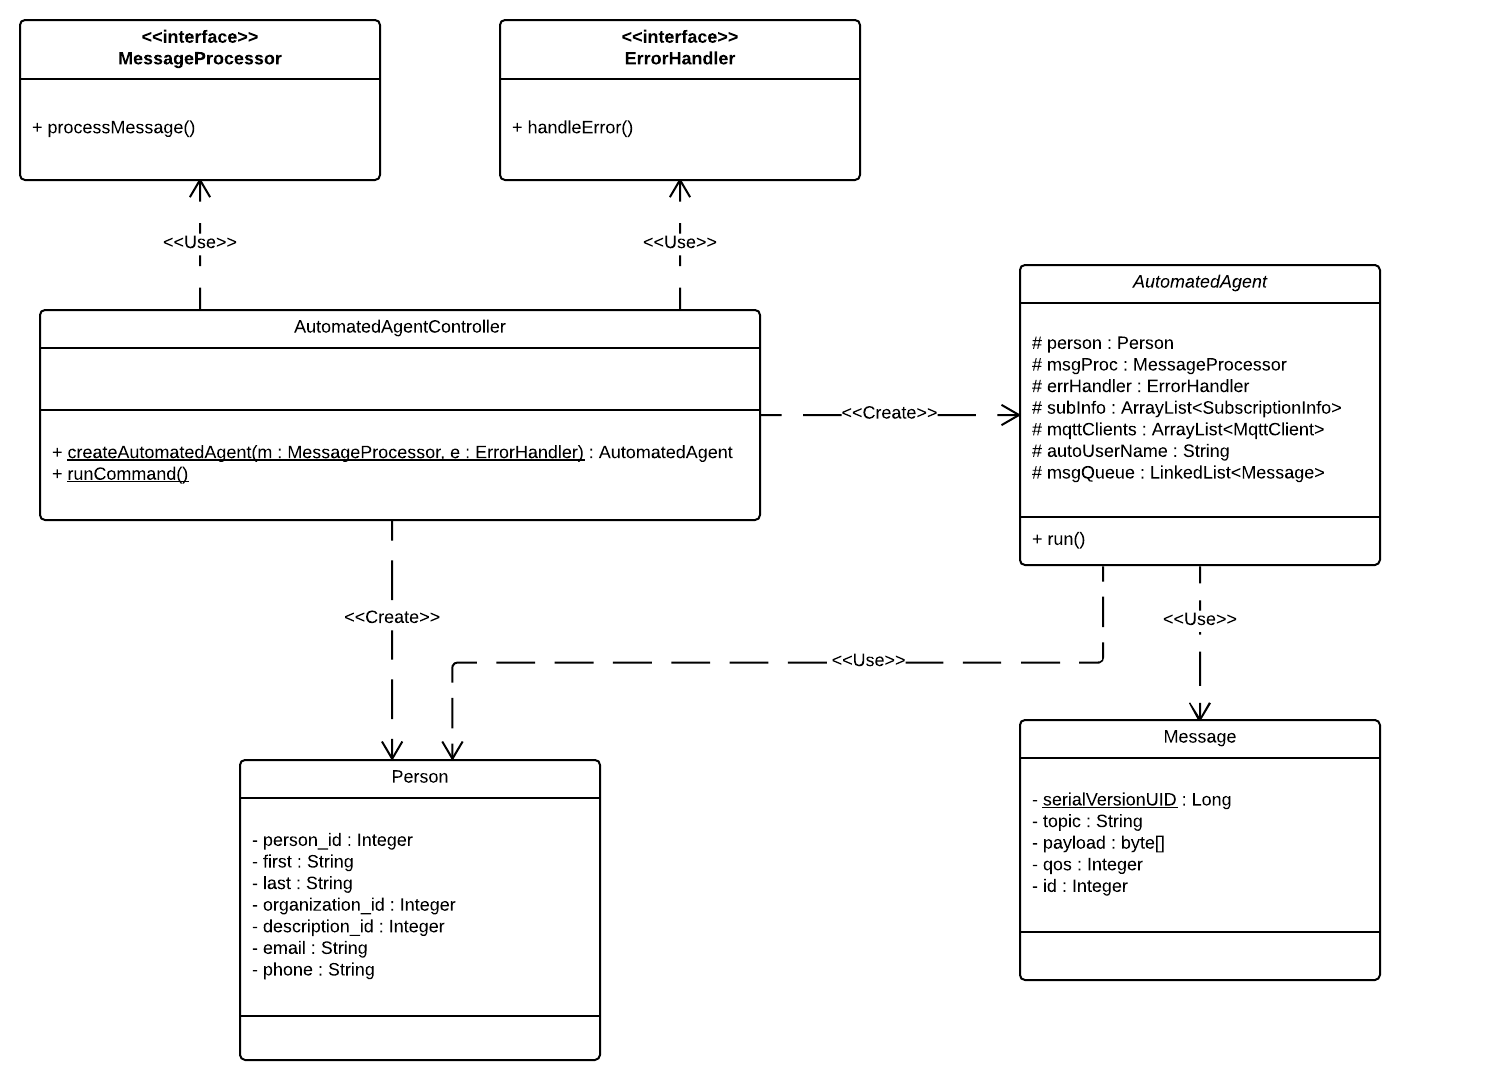
\includegraphics[width=\textwidth]{figures/automated_agent_class_diagram.png}
	\caption{A class diagram showing the composition of the agents and their relevant classes}
	\label{fig:automation_class_diagram}
\end{figure}

The text on each of the arrows denote a class using the item it is pointing to, or whether is is creating an instance of the item it is pointing to. The Automated User Controller class uses the Message Processor and Error Handler interfaces to create Automated User and Person objects. Each Automated User object can then use its Person object, the functionality in the Message class, and whatever functions that were passed in for the Message Processor and Error Handler to complete its tasks. A detailed example of the software classes showing how this software actually works is described in the next section.



%If a software application is given the data streams necessary to identify certain event conditions and the capability to make decisions, then the reconfiguration process can be automated, and performed in a quicker and more efficient way than if a human user were to do it. The Validation module and the user access control data schema work well for users and entities to perform reconfigurations. Because of this, designing an automated piece of reconfiguration software as an artificial user will allow the the reconfiguration to be governed by the same validation and user access control paradigm as human users.\\

%The software applications which autonomously monitor and reconfigure WiSARDs are called automated agents. It is important that these agents are designed an implemented in a way that respects the user access control paradigm so that they can safely and efficiently operate. Additionally, a modular approach to designing the agents is necessary to allow a wide variety of network management capabilities without being cumbersome to the developer.\\

% modular message processor
%The first piece of the automated agent is called the message processor. This component is responsible for acquiring data streams and fetching data so that the agent can analyze and make informed decisions. This component is the most modular piece of the automated agent, and is defined by a Java class whose objects are passed to the agent. The message processor in software is made using a Java 8 lambda expression, which allows it to be passed around as a first-class object \textbf{cite this}. 

%The message processor software can communicate with the PostgreSQL database as well as interact with MQTT brokers. This gives the developer the flexibility to access current data that has recently been sampled, but also lets the agents have access to archived data from the database for a diverse range of analyses. 

% agent uses same command and validation logic from previous chapter
%The second piece of the automated agent is the logic which generates commands to reconfigure WiSARDs based on whatever assessments resulted from the message processor. The flexible design of the Command Generation module allows the agent to utilize its functionality in the same way that a human user would be able. Additionally, the portion of the validation module which performs the safety validation checks can also be utilized by the agents in the same way that a human user can.\\


% need for validation and permission checking outside of the agent
%The user access control portion of the validation module is handled a bit differently than the safety validation check. Because users of the platform will eventually be creating their own agents, it is important for the user access validation to be checked separately, so that users will be less likely to exploit the permission system. This provides the motivation for a separate piece of software called the Automated Agent Controller.\\

%This piece of software is defined by a Java class which performs three functions. First, the controller takes in user login information as parameters. It logs in the user and verifies the identity of the automated agent against the permission entities in the database. Second, the controller looks at the message processor which it also is passed as a parameter. The controller validates that the user has sufficient privilege to access the data streams it will be monitoring. Finally, if the login and user access validations were successful, the controller will create an automated agent object. Once created, the agent object can run and autonomously manage the WiSARDs. 


% 6.3 Example Then just give the example code for MyAutomatedUser, AutomatedUser, and the interfaces

% Then end with a paragraph about how the design is good: it is simple and quick to create a user, it is flexible, etc...

\section{Example Agent}
% 3. Example description and code for a very simple agent
%	- flow of execution visual?%
Using the design described in the previous section, there are many different ways that an automated agent can be used to manage WiSARDs. The following code snippets and class definitions demonstrate how this functionality is used in practice.\\

Below is the class definition for the agent controller that handles authentication and creation of the agents.\\
% AutomatedUserController class
\lstinputlisting[language = java, firstline = 32, lastline=44]{AutomatedUser.java}
 
 
  This is the class definition for the agents. An instance of this class is created by the agent controller and returned. In the constructor, all of the necessary information to establish connections to MQTT message brokers as well as define the agent's behavior is passed in as a set of parameters. The run() method shows how an agent establishes its subscriptions with the MQTT brokers it will be listening to, and then waits for messages to arrive. Once messages arrive, they are given to the processMessage() method whose functionality was passed into the constructor as a lambda expression.\\
  
 % AutomatedUser class	
 \lstinputlisting[language = java, firstline = 64, lastline=132]{AutomatedUser.java}
 
 These are the definitions for the functional interfaces that allow lambda expressions to be passed to the agents to define their behavior.
 
 % Interfaces
 \lstinputlisting[language = java, firstline = 16, lastline=30]{AutomatedUser.java}
 
  This code snippet shows an example of how to utilize the classes defined above in a runnable program that uses automated agents. The comments demonstrate what code a user would need to add to customize their agent.\\ 	
 
 % using everything
 \lstinputlisting[language = java, firstline = 46, lastline=62]{AutomatedUser.java}
 

 	
%There are many different ways in which an automated agent can be used to manage WiSARDs in the WiSARDNet platform. For a practical example, assume a researcher desires to capture a set of high resolution soil moisture readings of rain events in a particular area, but does not want their WiSARD to sample at a high rate when there are no rain events. An automated agent could be used to identify pending storms from neighboring areas by monitoring their soil moisture data readings, and then preemptively updating the sampling rate of the WiSARDs at the region of interest.\\

%To create an automated agent with this functionality the steps described in the previous section need to be taken.

%\begin{itemize}
%	\item Define a Message Processor with the logic it will use to monitor the data streams of interest.
%	\item Create an ArrayList data structure of subscription objects with the connection information to the different sites it will be monitoring.
%	\item Create an Automated Agent Controller object
%	\item Use the Automated Agent Controller to create and authenticate an Automated Agent
%	\item Run the Automated agent.
%\end{itemize}

%\textbf{Show the code that defines a message processor}

%\textbf{Show the code that creates the arraylist of subscription objects as well as the class definition for subscription objects}

%\textbf{Show the code that creates the Automated Agent Controller and the Automated Agent as well as class definitions for both}

%\text{Show the code that runs the Agent and the logic it executes} % Results and Discussion

%% Chapter 7

\chapter{Conclusion and Future Work}
\label{Chapter 7}
%\head{}

% 7 Future Work and Conclusion
% - Describe what your work accomplished
% * Describe each module
% 	- what it accomplishes
%	- How it could be expanded for future work given its design

\section{Overview}
This work introduces new functionality into the WiSARDNet platform that enhances the usability of the system for researchers. Its design also provides a foundation for more features to be added in the future. This chapter summarizes the accomplishments of this thesis and assesses the impact each component has on the WiSARDNet platform and its users. Finally, this chapter discusses opportunities for future work. 

\section{Conclusions}
This work presents a design and implementation for adding network reconfiguration capabilities to the WiSARDNet platform according to the requirements established in Chapter 1. Each design requirement is listed below along with a description of how it was accomplished in this work.

\begin{itemize}
	\item \textbf{Implementation of an application that allows users to remotely identify and select sets of WSN nodes based on static and dynamic search criteria.} Wisard\_Browser\_Module fulfills this objective by allowing users to specify information that corresponds to a variety of WiSARD attributes that are both static and dynamic in nature. This module produces a set of WiSARDs that match the search criteria entered by the user. 

	\item \textbf{Implementation of an interface allowing users to enact behavioral changes in individual or groups of nodes.} This objective is satisfied by Cmd\_Generation\_Module that generates commands to reconfigure WiSARDs based on changes by the user. The extent to which a user can reconfigure the WiSARDs is governed by a user access control  and network safety check that is performed for every command that is generated.

	\item \textbf{Generalization of the reconfiguration software such that agents can monitor and reconfigure network nodes.} This is satisfied with the implementation of automated agents that are able to utilize Wisard\_Browser\_Module, Cmd\_Generation\_Module, and Validation\_Module to reconfigure WiSARDs in reaction to different events that can be specified for each agent. Additionally, automated agents are subject to the same user access control and validation rules as human users.
\end{itemize}


\section{Future Work}
WiSARDNet is a platform that supports complex distributed ecological experiments. In this work, the addition of user access control, remote reconfiguration, and the ability to automate reconfiguration adds valuable functionality to the WiSARDNet platform. It also provides a foundation supporting additional capabilities. 

\subsection{Stored Behaviors and Profiles}
The central paradigm of this thesis is that a WSN can be viewed as a database of heterogeneous behaviors, and that network reconfiguration can be achieved using a database approach. The process of network reconfiguration utilizes a command generator to build messages that invoke WSN configuration changes. A natural extension of this functionality would be for a user to have access to reconfiguration profiles, or groups of reconfiguration commands that produce a more complex defined behavior for a WiSARD. These profiles could be stored in a PostgreSQL data table, and could be selected and deployed to a set of WiSARDs.

One example is a low power profile that reduces the sampling rates of all transducers in a WiSARD. This profile could also change the WiSARD's role from a node that relays messages to other nodes into a leaf node that does not need to expend energy communicating with other nodes. Once operational, a user would have access to this profile that could then be executed via the commands it encapsulates. Additionally, profiles could be governed by the user access control system, due to the generalized nature of the user access control schema. An extension of the PermissionResource table to include profiles would allow a permission entity to be granted access to specific profiles. 

\subsection{OTA Reprogramming}
Currently, new firmware versions must be physically uploaded to the WiSARDs because there is no over-the-air (OTA) reprogramming capability for the WiSARDs. The software implemented for this thesis could be expanded to support OTA reprogramming. The compiled source code for a new firmware version could be broken down into a series of messages, where each message payload contains a numbered piece of the new firmware. These messages could be sent sequentially to the intended WiSARD; once the WiSARD has received all of the messages, it could begin to overwrite the existing firmware in flash memory with the new firmware.

Implementing these features would not be a trivial task. OTA reprogramming would require expanding the command generation with features that would support breaking down a file containing a new firmware into many messages, numbering these messages, and sending these messages to the intended WiSARD. Additionally the firmware on WiSARDs would need to be upgraded to support these behaviors as well. The WiSARD would need to be able to recognize that each message is a piece of a new firmware, and would need to store that piece of the message. Additionally, the WiSARD would need to verify that it has received all of the messages correctly, assemble the firmware pieces from each message into the entire file, and then overwrite the existing firmware with the new version. The process of overwriting the old firmware with the new one would also need to have a way to revert back to the old firmware if the new firmware was unable to be correctly downloaded or stored.

OTA reprogramming would require all of these new features, but the work of this thesis provides a foundation for these features to be built upon. 

\subsection{Creation of Complex Automated Agents}
The addition of automated agents to the WiSARDNet system provides a way for the WSNs to be monitored and reconfigured in real time based on different events that a developer or researcher must specify for each agent. The use case described in Chapter 6 is a fairly simple example which manages the sampling rate of a WiSARD based on the time of day, but the system supports complex agents that monitor and reconfigure large numbers of WiSARDs in response to many different events. The agents are designed to have access to all of the monitoring and reconfiguration features that a human user does, so any improvements or additions to the modules such as the ones described in the previous sections would also benefit the agents in expanding their capabilities. Everything is in place for a user to build a complex agent by following the example code in Chapter 6.

\subsection{Improved User Interface}
As is the case with many software systems, there are plenty of opportunities for improvements to be made to the user interface. The user interface for the WiSARD Browser and Command Generation Module presents users with a simple way to enter WiSARD search criteria and specify changes. This can be improved with the inclusion of a geographic map that allows a user to view all of the WiSARDs that he/she has permission to reconfigure. Users with experiments spanning large geographic regions would have an easier time visualizing the effects of a reconfiguration if they had access to a user interface that displayed WiSARDs in this way.

Another opportunity for improvement is a user interface that lets a user build an automated agent visually, rather than requiring that he/she develop an agent by programming it directly. This would make automating network reconfiguration much more accessible to researchers without sufficient Java programming experience. This would require generalizing the agent code and allowing boiler-plate features to be specified and populated from either a form or some other type of user input. Additionally, allowing users to edit and modify agents from this user interface would also be beneficial.

\subsection{Integration of Other IoT Platforms}
IoT devices are growing in number every day, and because of this there are many other WSN platforms and management solutions being developed and used, such as Amazon Web Services (AWS IoT). AWS IoT is a software platform which provide cloud management services to IoT devices. There is great potential for the work of this thesis to be adapted for use in another WSN platform such as AWS IoT.

Integration of the work of this thesis into another platform would not be a trivial task, but there are a couple of foundational similarities between AWS IoT and parts of WiSARDNet that present an opportunity for future work that is worth exploring. For example, AWS IoT uses the  MQTT as a middleware solution for connecting IoT devices to the AWS cloud. Portions of the WiSARDNet publish/subscribe clients (Raw Data Fetcher and WiSARD Client) could be adapted to allow garden servers to connect to the AWS cloud as opposed to the WiSARDNet RTDC. Once accomplished, Wisard\_Browser\_Module, Cmd\_Generation\_Module, and Validation\_Module could then be adapted to provide their WiSARD reconfiguration functionality with the tools that the AWS IoT platform provides.

The largest obstacle to an integration such as this is the reliance that WiSARDNet has on a relational database. AWS IoT provides database services to networked devices using DynamoDB, a non-relational database. Many of the abstractions used to manage WiSARDs and experiments in WiSARDNet would not translate easily to a non-relational database paradigm and would require a different approach. Additionally, Wisard\_Browser\_Module and Validation\_Module were designed in such a way that they take advantages of the relational database paradigm used in WiSARDNet. Using these modules in a platform like AWS would require the code be modified to use a different paradigm.

Once the code has been modified to support the new paradigm however, automated agents could be easily implemented to reconfigure WiSARDs using AWS IoT event triggers which allow for actions to be taken in response to the analysis of incoming data streams. The event trigger paradigm used in AWS IoT is similar to the design approach taken for automated agents in this work, and therefore the control logic could translate without extensive reorganization.

 % Conclusion

%% ----------------------------------------------------------------
% Now begin the Appendices, including them as separate files


\clearpage
\backmatter
\addtocontents{toc}{\vspace{2em}}  % Add a gap in the Contents, for aesthetics

\appendix
% Appendix

\chapter{Appendix}
\label{Appendix:agent}
\lhead{}

The framework provided in this thesis allows a user to create their own automated agent to reconfigure WiSARDs or control experiments. The creation of an automated agent for use with WiSARDNet requires Java programming experience as well as familiarity with a command line interface. Additionally, a WiSARDNet system administrator will need to create an account for the user making the agent.

First, you will need to create a new Java project in the editor of your choice. Eclipse was used in the work of this thesis and is recommended for the creation of automated agents. To utilize the automated agent framework developed in the work of this thesis, you will need a few open source support libraries to be added to your project.

\begin{itemize}
	\item The PostgreSQL JDBC Driver
	\item The Java Commons Codec 
	\item The Eclipse Paho MQTT Driver
\end{itemize}

These libraries will allow you to connect to the WiSARDNet PostgreSQL database, connect to a WiSARDNet MQTT broker, create publish and subscribe clients, and parse message packets. Additionally, you will need to include the WiSARDNet Helpers, Interfaces, and Utilities support libraries in your project. These support libraries contain a variety of Java classes and interfaces that enable interaction with the different WiSARDNet systems. These include the AutomatedAgent and AutomatedAgentController classes discussed in Chapter 6. 

%\section{Writing the Code}
To create an agent, you will need to create Java file that defines a class. There are three critical components your class will need to have.

\begin{itemize}
	\item A main method
	\item A MessageProcessor
	\item An ErrorHandler
\end{itemize}

The main method is needed so that the agent will be runnable as a command line program. The entire class file for the greenhouse experiment agent described in Chapter is shown in the code sample below. This class file provides an example for how each of these software pieces can be approached.

\lstinputlisting[language = java, firstline = 1, lastline=144]{appendix_agent_example.java}

The main method needs username and password Strings as command line input parameters; this is necessary for the agent to be authenticated. Within the main method, you need to define an ArrayList data structure of SubscriptionInfo objects. These objects must contain the connection information necessary to subscribe to a set of WiSARD streams from a particular MQTT broker. You will need to make one SubscriptionInfo object for every broker you wish to receive data from. Next, you will need to define a MessageProcessor and an ErrorHandler. The MessageProcessor is a lambda expression which contains the logic that an agent will use to process MQTT messages. The ErrorHandler is a lambda expression that defines how the agent will handle the different types of exceptions that can occur.

To complete your agent, you will need to place two function calls at the end of your main method. First, you will need to call the createAutomatedAgent static method from the AutomatedAgentController class, and pass it the username, password, SubscriptionInfo ArrayList, MessageProcessor, and ErrorHandler variables as input parameters. The method signature in the AutomatedAgentController class file shows exactly how these parameters need to be passed. The results of this static method call should be assigned to a variable. In this example, the variable \verb|agent| is used to reference the created object. Finally, A new \verb|Thread()| object needs to be created and passed \verb|agent| as a parameter and the \verb|start()| method needs to be called. Once all of these things are in the class file, the agent program can be finalized and run.

Once the code is written for the automated agent, the files and support libraries need to be exported as a runnable JAR file. If prompted by your development editor, the required libraries should be packaged with your code into the JAR file. 

%% ----------------------------------------------------------------
\nocite{*}
%\label{Bibliography}
%\lhead{\emph{Bibliography}}  % Change the left side page header to "Bibliography"
%\bibliographystyle{IEEEtrans}  % Use the "unsrtnat" BibTeX style for formatting the Bibliography
\bibliographystyle{ieeetr}
\bibliography{Bibliography}  % The references (bibliography) information are stored in the file named "Bibliography.bib"


\end{document}  % The End
%% ----------------------------------------------------------------